\documentclass[11pt,a4paper]{article}

% =========================================================
% PACKAGES
% =========================================================
\usepackage[utf8]{inputenc}
\usepackage[T1]{fontenc}
\usepackage{lmodern}
\usepackage[a4paper,margin=2.2cm]{geometry}

\usepackage{amsmath,amssymb}
\usepackage{booktabs}
\usepackage{array}
\usepackage{longtable}
\usepackage{multirow}
\usepackage{graphicx}
\usepackage{float}
\usepackage{caption}
\usepackage{subcaption}
\usepackage{xcolor}
\usepackage{enumitem}
\usepackage{microtype}
\usepackage{setspace}
\usepackage{titlesec}
\usepackage{fancyhdr}

\usepackage[hidelinks]{hyperref}
\usepackage{bookmark}

\usepackage{tikz}
\usepackage{pgfplots}
\usepackage{adjustbox}
\usepackage{tabularx}

\usetikzlibrary{shapes.geometric,shapes.misc,arrows.meta,positioning,calc}

\pgfplotsset{compat=1.18}

% =========================================================
% DOCUMENT SETTINGS
% =========================================================
\onehalfspacing
\setlength{\parindent}{0pt}
\setlength{\parskip}{5pt}

\hypersetup{
    colorlinks=true,
    linkcolor=black,
    citecolor=black,
    urlcolor=blue,
    pdftitle={Data-Driven Customer Analytics for E-Commerce Decision Making},
    pdfauthor={Mahdiyeh Mirzaei}
}

% =========================================================
% HEADER / FOOTER
% =========================================================
\pagestyle{fancy}
\fancyhf{}
\lhead{\small Customer Analytics for E-Commerce}
\rhead{\small Mahdiyeh Mirzaei}
\cfoot{\thepage}
\renewcommand{\headrulewidth}{0.4pt}

% =========================================================
% SECTION STYLE
% =========================================================
\titleformat{\section}
{\large\bfseries}
{\thesection.}
{0.6em}
{}

\titleformat{\subsection}
{\normalsize\bfseries}
{\thesubsection.}
{0.6em}
{}

\titleformat{\subsubsection}
{\normalsize\itshape}
{\thesubsubsection.}
{0.6em}
{}

\titlespacing*{\section}{0pt}{18pt}{8pt}
\titlespacing*{\subsection}{0pt}{12pt}{5pt}

% =========================================================
% TABLE SETTINGS
% =========================================================
\captionsetup{
    font=small,
    labelfont=bf,
    justification=centering
}

\renewcommand{\arraystretch}{1.2}

% =========================================================
% CUSTOM COMMANDS
% =========================================================
\newcommand{\Hnull}{H_{0}}
\newcommand{\Halt}{H_{1}}

% =========================================================
% DOCUMENT
% =========================================================
\graphicspath{{customer_article_figures/}}

\begin{document}

% =========================================================
% TITLE PAGE
% =========================================================

\begin{titlepage}
\centering

\vspace*{1.5cm}

{\Large\bfseries Data-Driven Customer Analytics for E-Commerce Decision Making\par}

\vspace{0.7cm}

{\large\itshape An Integrated Statistical and Machine-Learning Approach to Customer Value, Churn Risk, Segmentation, and Marketing Optimization\par}

\vspace{1.8cm}

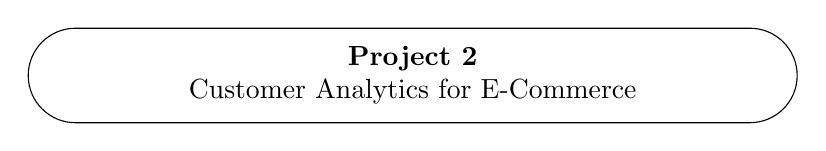
\begin{tikzpicture}
\node[
    draw,
    rounded rectangle,
    minimum width=10cm,
    minimum height=1.2cm,
    align=center
]
{
\textbf{Project 2}\\
Customer Analytics for E-Commerce
};
\end{tikzpicture}

\vfill

{\large
\textbf{Author}\\[0.2cm]
Mahdiyeh Mirzaei
\par}

\vspace{0.5cm}

{\large
\textbf{Team / Community}\\[0.2cm]
StudyBuild Community
\par}

\vspace{0.5cm}

\href{https://github.com/mahdiyeh-mirzaei-v2}
{github.com/mahdiyeh-mirzaei-v2}

\vspace{0.15cm}

\href{https://github.com/StudyBuildCommunity}
{github.com/StudyBuildCommunity}

\vfill

{\large
\textbf{2026}
\par}

\end{titlepage}

% =========================================================
% ABSTRACT
% =========================================================

\section*{Abstract}
\addcontentsline{toc}{section}{Abstract}

This study presents an integrated customer analytics framework for an e-commerce company using statistical analysis, unsupervised learning, and supervised machine learning. The analytical dataset contains 60 customers and 26 original variables covering demographic, transactional, behavioral, and satisfaction-related characteristics. The methodology combines exploratory data analysis, descriptive statistics, normality testing, Interquartile Range (IQR)-based outlier detection, Spearman rank correlation, customer value scoring, K-Means clustering, non-parametric hypothesis testing, churn-risk classification, and predictive modeling.

The results indicate substantial heterogeneity in customer economic value. Customers were divided into three equally sized value groups, including 20 High-Value, 20 Medium-Value, and 20 Low-Value customers. A total of 36 customers, corresponding to 60\% of the sample, were classified as churn-risk customers using an inactivity threshold of more than 180 days. Importantly, 12 customers were simultaneously classified as High Value and Churn Risk, identifying a strategically critical retention group.

K-Means clustering identified three behavioral segments. The most valuable cluster consisted of only six customers but exhibited an average total spending of approximately 14,188.76. The Kruskal--Wallis test confirmed statistically significant differences in spending distributions across clusters ($H=16.109$, $p=0.000318$).

The discount analysis did not identify a statistically significant difference in spending between customers using discounts and those not using discounts. The Mann--Whitney U test resulted in $U=391$ and $p=0.4512$. The machine-learning analysis also produced limited predictive performance, with mean cross-validated ROC-AUC values of approximately 0.564 for Logistic Regression and 0.478 for Random Forest.

At the geographical level, Mashhad generated the highest observed total revenue of approximately 64,118.44 and obtained the highest marketing opportunity score. Based on these findings, the study recommends prioritizing high-value churn-risk customers, increasing average order value among frequent low-basket customers, and validating marketing investment in Mashhad through controlled experimentation.

\textbf{Keywords:} Customer Analytics; E-Commerce; Customer Value; Churn Risk; K-Means; Logistic Regression; Random Forest; Spearman Correlation; Non-Parametric Statistics; Marketing Analytics.

% =========================================================
% TABLE OF CONTENTS
% =========================================================

\newpage
\tableofcontents
\newpage

% =========================================================
% 1 INTRODUCTION
% =========================================================

\section{Introduction}

The rapid expansion of e-commerce has created large volumes of customer-level data containing information about purchasing behavior, transaction value, customer satisfaction, discounts, returns, and demographic characteristics. The availability of such data provides organizations with an opportunity to move from intuition-based marketing toward evidence-based decision making.

However, raw customer data do not directly provide managerial insight. Organizations must identify economically valuable customers, recognize inactive or potentially lost customers, understand heterogeneous behavioral patterns, and determine where marketing resources are most likely to generate incremental value.

The central research question of this project is:

\begin{quote}
\textit{How can customer-level behavioral and transactional data be transformed into statistically supported and actionable strategies for improving customer retention, revenue generation, and marketing efficiency?}
\end{quote}

The analysis addresses five principal managerial questions:

\begin{enumerate}[label=\arabic*.]
    \item Which customers generate the greatest economic value?
    \item Which customers are potentially at risk of becoming inactive?
    \item Which customer segments exhibit distinct purchasing behavior?
    \item Which geographical market provides the strongest marketing opportunity?
    \item Is discount usage associated with higher customer spending?
\end{enumerate}

In addition, supervised machine-learning models are evaluated to determine whether customer characteristics provide useful information for identifying churn-risk customers.

The purpose of this study is therefore not merely descriptive. The analytical framework explicitly connects statistical evidence to business decisions.

% =========================================================
% 2 DATA
% =========================================================

\section{Data Description and Preparation}

\subsection{Dataset Overview}

The final analytical dataset contains 60 customers and 26 original variables. The variables represent demographic, transactional, behavioral, and customer-satisfaction characteristics.

Important variables include:

\begin{itemize}
    \item \texttt{customer\_id}
    \item \texttt{age}
    \item \texttt{city}
    \item \texttt{province}
    \item \texttt{membership\_tier}
    \item \texttt{purchase\_count}
    \item \texttt{avg\_order\_value}
    \item \texttt{total\_spending}
    \item \texttt{last\_purchase\_days}
    \item \texttt{discount\_used}
    \item \texttt{returned\_items}
    \item \texttt{satisfaction\_score}
\end{itemize}

Several analytical variables were subsequently engineered, including:

\begin{itemize}
    \item Customer Value Score
    \item Customer Value Segment
    \item Churn Risk
    \item Churn Risk Label
    \item K-Means Cluster
\end{itemize}

\subsection{Data Quality}

The data-quality audit identified no duplicate observations. Therefore,

\[
N=60,
\qquad
\text{Duplicate Rows}=0.
\]

Table~\ref{tab:dataset_summary} summarizes the main properties of the analytical dataset.

\begin{table}[H]
\centering
\caption{Summary of the analytical dataset}
\label{tab:dataset_summary}
\begin{tabular}{lr}
\toprule
\textbf{Property} & \textbf{Value}\\
\midrule
Customers & 60\\
Original variables & 26\\
Final analytical variables & 31\\
Duplicate rows & 0\\
Active customers & 24\\
Churn-risk customers & 36\\
High-value customers & 20\\
Medium-value customers & 20\\
Low-value customers & 20\\
K-Means clusters & 3\\
\bottomrule
\end{tabular}
\end{table}

% =========================================================
% 3 METHODOLOGY
% =========================================================


% =========================================================
\section{Theoretical and Statistical Foundations}
\label{sec:theory}

This section establishes the statistical theory underlying the empirical
analysis. The framework is aligned with the procedures implemented in the
project: descriptive statistics, standardization, distributional
diagnostics, rank correlation, non-parametric inference, bootstrap
inference, customer-value scoring, clustering, classification, and
predictive discrimination \cite{cohen,efron,hastie,james}.

\subsection{Descriptive Statistics}

For a quantitative variable $X=(X_1,\ldots,X_n)$, the arithmetic mean is
\begin{equation}
\bar X=\frac{1}{n}\sum_{i=1}^{n}X_i,
\end{equation}
and the sample variance and standard deviation are
\begin{equation}
s^2=\frac{1}{n-1}\sum_{i=1}^{n}(X_i-\bar X)^2,
\qquad
s=\sqrt{s^2}.
\end{equation}

The interquartile range is
\begin{equation}
IQR=Q_3-Q_1,
\end{equation}
with conventional outlier-screening bounds
\begin{equation}
L=Q_1-1.5IQR,\qquad U=Q_3+1.5IQR.
\end{equation}
Values outside $[L,U]$ are potential statistical outliers, but they are
not automatically erroneous because extreme customers may be economically
important.

\subsection{Standardization and Z-Scores}

Standardization places variables on a common scale:
\begin{equation}
z_i=\frac{x_i-\bar x}{s}.
\end{equation}
This transformation is important for composite scoring and distance-based
clustering because it prevents variables with larger measurement scales
from dominating the analysis.

\subsection{Shapiro--Wilk Normality Test}

The Shapiro--Wilk statistic is
\begin{equation}
W=
\frac{\left(\sum_{i=1}^{n}a_i x_{(i)}\right)^2}
{\sum_{i=1}^{n}(x_i-\bar{x})^2},
\end{equation}
where $x_{(i)}$ are ordered observations and $a_i$ are coefficients derived
from expected normal order statistics \cite{shapiro}. The hypotheses are
\begin{equation}
H_0:X\sim\mathcal N(\mu,\sigma^2),
\qquad
H_1:X\not\sim\mathcal N(\mu,\sigma^2).
\end{equation}
At $\alpha=0.05$, $p<0.05$ provides evidence against normality. The project
found strong non-normality for total spending and several other variables,
which motivates robust and non-parametric procedures.

\subsection{Spearman Rank Correlation}

Spearman's coefficient measures monotonic association without requiring
normality \cite{spearman}:
\begin{equation}
\rho_s=
1-\frac{6\sum_{i=1}^{n}d_i^2}{n(n^2-1)},
\end{equation}
where $d_i$ is the difference between the two ranks for observation $i$.
The coefficient satisfies $-1\leq\rho_s\leq1$. Association should not be
interpreted as causation.

\subsection{Customer Value Score}

The project defines a weighted customer-value index:
\begin{equation}
CVS_i=
0.50Z(TS_i)+0.30Z(PC_i)+0.20Z(AOV_i),
\end{equation}
where $TS$ is total spending, $PC$ is purchase count, and $AOV$ is average
order value. The weights sum to one:
\begin{equation}
0.50+0.30+0.20=1.
\end{equation}
The score is subsequently divided into empirical quantile groups.

\subsection{Recency-Based Churn Risk}

The operational churn indicator is
\begin{equation}
C_i=
\begin{cases}
1,&L_i>180,\\
0,&L_i\leq180,
\end{cases}
\end{equation}
where $L_i$ is days since last purchase. The observed risk rate is
\begin{equation}
\hat p_{\mathrm{risk}}=
\frac{\sum_{i=1}^{n}C_i}{n}.
\end{equation}
This is an inactivity rule, not a future-event survival probability.

\subsection{Mann--Whitney U Test}

For two independent groups, the Mann--Whitney U statistic is based on
pooled ranks \cite{mannwhitney}:
\begin{equation}
U_1=R_1-\frac{n_1(n_1+1)}{2}.
\end{equation}
The hypotheses are
\begin{equation}
H_0:F_1(x)=F_2(x)
\quad\text{versus}\quad
H_1:F_1(x)\neq F_2(x).
\end{equation}
For discount usage, the project obtained $U=391$ and $p=0.4512$.

\subsection{Effect Size: Cohen's $d$}

For two independent groups,
\begin{equation}
d=\frac{\bar X_1-\bar X_2}{s_p},
\end{equation}
where
\begin{equation}
s_p=
\sqrt{
\frac{(n_1-1)s_1^2+(n_2-1)s_2^2}
{n_1+n_2-2}
}.
\end{equation}
The reported discount effect was approximately $d=-0.022$, indicating a
negligible standardized difference \cite{cohen}.

\subsection{Bootstrap Confidence Interval}

Bootstrap inference repeatedly resamples observations with replacement
\cite{efron}. For a mean difference $\Delta=\bar X_1-\bar X_2$,
bootstrap replications $\Delta^{*(b)}$ yield a percentile interval
\begin{equation}
CI_{0.95}=
\left[
Q_{0.025}(\Delta^*),
Q_{0.975}(\Delta^*)
\right].
\end{equation}
The project used $B=5000$ replications and obtained
$[-2146.19,2400.88]$ for the mean spending difference.

\subsection{K-Means Clustering}

K-Means minimizes within-cluster squared Euclidean distance
\cite{kmeans}:
\begin{equation}
\min_{\mathcal C}
\sum_{k=1}^{K}\sum_{x_i\in C_k}
\lVert x_i-\mu_k\rVert_2^2.
\end{equation}
The centroid is
\begin{equation}
\mu_k=
\frac{1}{|C_k|}\sum_{x_i\in C_k}x_i.
\end{equation}

\subsection{Silhouette Coefficient}

For observation $i$, the silhouette coefficient is
\begin{equation}
s(i)=
\frac{b(i)-a(i)}
{\max\{a(i),b(i)\}},
\end{equation}
where $a(i)$ is mean within-cluster distance and $b(i)$ is the smallest
mean distance to another cluster \cite{silhouette}. The selected
solution had $K=3$ and silhouette score $0.316$, indicating moderate
separation.

\subsection{Kruskal--Wallis Test}

For $k$ independent groups, the Kruskal--Wallis statistic is
\begin{equation}
H=
\frac{12}{N(N+1)}
\sum_{j=1}^{k}\frac{R_j^2}{n_j}
-3(N+1),
\end{equation}
where $R_j$ is the rank sum in group $j$ \cite{kruskal}. The project
obtained
\begin{equation}
H=16.109,\qquad p=0.000318,
\end{equation}
supporting statistically significant differences among the clusters.

\subsection{Logistic Regression}

For binary churn-risk prediction,
\begin{equation}
P(Y_i=1\mid X_i)=
\frac{1}{1+\exp(-\eta_i)},
\end{equation}
with
\begin{equation}
\eta_i=\beta_0+\sum_{j=1}^{p}\beta_jX_{ij}.
\end{equation}
Equivalently,
\begin{equation}
\log\left(\frac{P(Y_i=1\mid X_i)}
{1-P(Y_i=1\mid X_i)}\right)
=\beta_0+\sum_{j=1}^{p}\beta_jX_{ij}.
\end{equation}

\subsection{Random Forest}

Random Forest is an ensemble of randomized decision trees
\cite{breiman}. A simplified classification representation is
\begin{equation}
\hat f(x)=\operatorname{mode}\{\hat f_b(x)\}_{b=1}^{B}.
\end{equation}
Feature importance describes predictive contribution within the fitted
ensemble and should not be interpreted as causal influence.

\subsection{ROC--AUC}

The true-positive and false-positive rates are
\begin{equation}
TPR=\frac{TP}{TP+FN},
\qquad
FPR=\frac{FP}{FP+TN}.
\end{equation}
ROC--AUC can be interpreted as
\begin{equation}
AUC=P(s(X^+)>s(X^-)).
\end{equation}
The reported mean cross-validated values were $0.564$ for Logistic
Regression and $0.478$ for Random Forest, indicating weak discrimination.

\subsection{Statistical Decision Rule}

The analysis adopts
\begin{equation}
\alpha=0.05.
\end{equation}
The inferential rule is
\begin{equation}
p<\alpha\Rightarrow\text{Reject }H_0,
\qquad
p\geq\alpha\Rightarrow\text{Fail to reject }H_0.
\end{equation}
Failure to reject a null hypothesis is not proof of equality; it indicates
that the available evidence is insufficient to reject the null under the
given sample and design.


\section{Data Quality Assessment}




The first stage consisted of structural and logical quality checks.
The dataset contained 60 customers and no duplicate records. The principal
analytical variables did not contain material missingness that prevented
the planned analyses.

A consistency check compared observed total spending with the expected
amount implied by purchase count and average order value:

\begin{equation}
E_i = \text{PurchaseCount}_i \times \text{AOV}_i.
\end{equation}

Two observations required additional review. Customer 1030 had observed
total spending of 25,000.00 compared with an expected value of approximately
4,079.14, producing a discrepancy of about 20,920.86. Customer 1040 had
observed spending of 126.00 compared with an expected value of approximately
1,280.44, producing a discrepancy of about 1,154.44.

These observations should be validated against the underlying transaction
system before the data are used for financial reconciliation or automated
decision rules.

Six records were also flagged for review in the returned-items analysis.
Customers requiring review had substantially lower mean spending
(596.10) and lower mean satisfaction (2.50) than customers without the
flag (mean spending 4,040.29; mean satisfaction 3.04). This pattern
suggests that return-related anomalies may also be associated with weaker
customer experience.

% =========================================================

\section{Descriptive Statistical Analysis}

The total observed revenue was 221,752.15, with a mean customer spending
of approximately 3,695.87 and a mean AOV of approximately 213.16.
The mean purchase count was approximately 17.38 transactions per customer.

The distribution of customer spending was highly heterogeneous. The
largest spending values were substantially above the central tendency,
which is consistent with the observed non-normal distribution and
motivates the use of robust and non-parametric procedures.

\section{Analytical Framework and Methodology}

The complete analytical workflow is illustrated in Figure~\ref{fig:workflow}.

\begin{figure}[H]
\centering
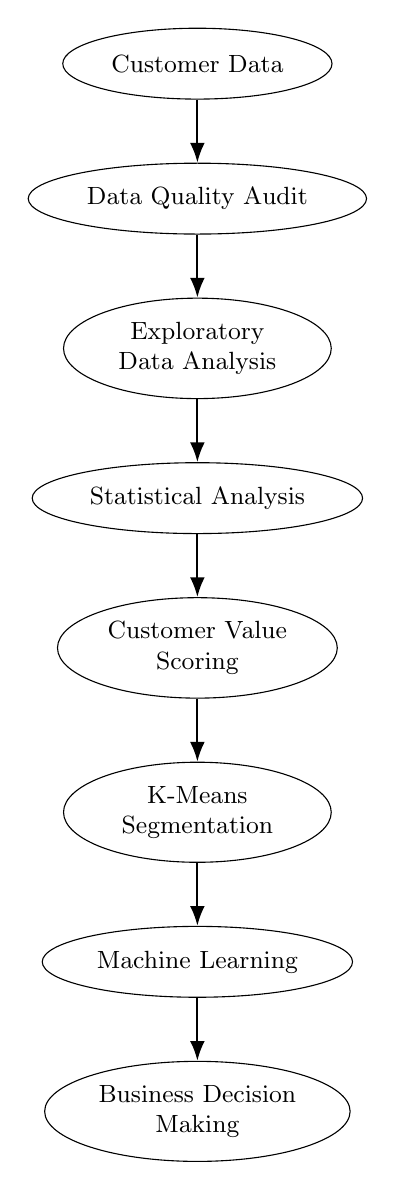
\begin{tikzpicture}[
node distance=0.8cm,
process/.style={
    draw,
    ellipse,
    minimum width=3.4cm,
    minimum height=0.9cm,
    align=center,
    font=\small
},
arrow/.style={
    -{Latex[length=2.5mm]},
    thick
}
]

\node[process] (data) {Customer Data};

\node[process, below=of data] (quality)
{Data Quality Audit};

\node[process, below=of quality] (eda)
{Exploratory\\Data Analysis};

\node[process, below=of eda] (stats)
{Statistical Analysis};

\node[process, below=of stats] (value)
{Customer Value\\Scoring};

\node[process, below=of value] (cluster)
{K-Means\\Segmentation};

\node[process, below=of cluster] (ml)
{Machine Learning};

\node[process, below=of ml] (business)
{Business Decision\\Making};

\draw[arrow] (data) -- (quality);
\draw[arrow] (quality) -- (eda);
\draw[arrow] (eda) -- (stats);
\draw[arrow] (stats) -- (value);
\draw[arrow] (value) -- (cluster);
\draw[arrow] (cluster) -- (ml);
\draw[arrow] (ml) -- (business);

\end{tikzpicture}
\caption{Integrated analytical framework used in the study}
\label{fig:workflow}
\end{figure}

The workflow combines descriptive, inferential, unsupervised, and supervised analytical techniques.

The main Python libraries used in the project include:

\begin{itemize}
    \item pandas
    \item NumPy
    \item SciPy
    \item scikit-learn
    \item matplotlib
    \item seaborn
    \item openpyxl
    \item joblib
\end{itemize}

% =========================================================
% 4 EDA
% =========================================================

\section{Exploratory Data Analysis}

Exploratory Data Analysis (EDA) was performed to characterize the distributions of customer age, purchase frequency, average order value, total spending, inactivity, and satisfaction.

Because the sample contains only 60 observations, numerical summaries were considered together with distributional diagnostics and graphical inspection.

The main numerical variables used throughout the analysis were:

\begin{itemize}
    \item Age
    \item Purchase Count
    \item Average Order Value
    \item Total Spending
    \item Last Purchase Days
    \item Satisfaction Score
\end{itemize}

The distributions indicate substantial heterogeneity, particularly in total spending and purchase behavior.

% =========================================================
% 5 NORMALITY
% =========================================================

\section{Normality and Outlier Analysis}

\subsection{Normality Testing}

The Shapiro--Wilk test was applied to assess the normality of the main numerical variables.

The null hypothesis was:

\[
\Hnull:\quad X \sim \text{Normal Distribution}.
\]

The alternative hypothesis was:

\[
\Halt:\quad X \not\sim \text{Normal Distribution}.
\]

The results are presented in Table~\ref{tab:normality_detailed}.

\begin{table}[H]
\centering
\caption{Shapiro--Wilk normality test}
\label{tab:normality_detailed}
\begin{tabular}{lcc}
\toprule
\textbf{Variable} & \textbf{W} & \textbf{p-value}\\
\midrule
Age & 0.938 & 0.004\\
Purchase Count & 0.957 & 0.033\\
Average Order Value & 0.915 & $<0.001$\\
Total Spending & 0.708 & $<0.001$\\
Last Purchase Days & 0.970 & 0.142\\
Satisfaction Score & 0.879 & $<0.001$\\
\bottomrule
\end{tabular}
\end{table}

At the 5\% significance level, most variables reject the normality hypothesis. Consequently, non-parametric statistical procedures are preferred for inferential comparisons.

\subsection{Outlier Detection}

Outliers were investigated using the Interquartile Range (IQR) criterion:

\[
IQR=Q_3-Q_1.
\]

The lower and upper bounds are defined as:

\[
L=Q_1-1.5(IQR),
\]

\[
U=Q_3+1.5(IQR).
\]

Observations outside $[L,U]$ are potential statistical outliers.

High-spending observations were not automatically removed because they may represent genuine economically important customers.

For example, Customer 1030 has:

\begin{align}
\text{Total Spending} &= 25,000,\\
\text{Purchase Count} &= 26,\\
\text{Last Purchase Days} &= 340.
\end{align}

This observation is statistically unusual but potentially highly valuable from a managerial perspective.

% =========================================================
% 6 CORRELATION
% =========================================================

\section{Correlation Analysis}

Because several variables exhibited non-normal distributions, Spearman's rank correlation coefficient was used.

Spearman's coefficient is defined as:

\[
\rho_s =
1-
\frac{6\sum d_i^2}{n(n^2-1)},
\]

where $d_i$ represents the difference between the ranks of the two variables for observation $i$.

The strongest relationships are summarized in Table~\ref{tab:correlation}.

\begin{table}[H]
\centering
\caption{Selected Spearman rank correlations}
\label{tab:correlation}
\begin{tabular}{lc}
\toprule
\textbf{Variable Pair} & \boldmath$\rho_s$\\
\midrule
Purchase Count -- Total Spending & 0.613\\
Average Order Value -- Total Spending & 0.434\\
Last Purchase Days -- Satisfaction & -0.293\\
Age -- Purchase Count & 0.265\\
\bottomrule
\end{tabular}
\end{table}

The strongest association was observed between Purchase Count and Total Spending:

\[
\rho_s=0.613.
\]

This indicates a moderate positive monotonic relationship, suggesting that customers who purchase more frequently tend to generate greater cumulative spending.

Nevertheless, correlation does not imply causation.

% =========================================================
% 7 CUSTOMER VALUE
% =========================================================

\section{Customer Value Analysis}

\begin{figure}[H]
\centering
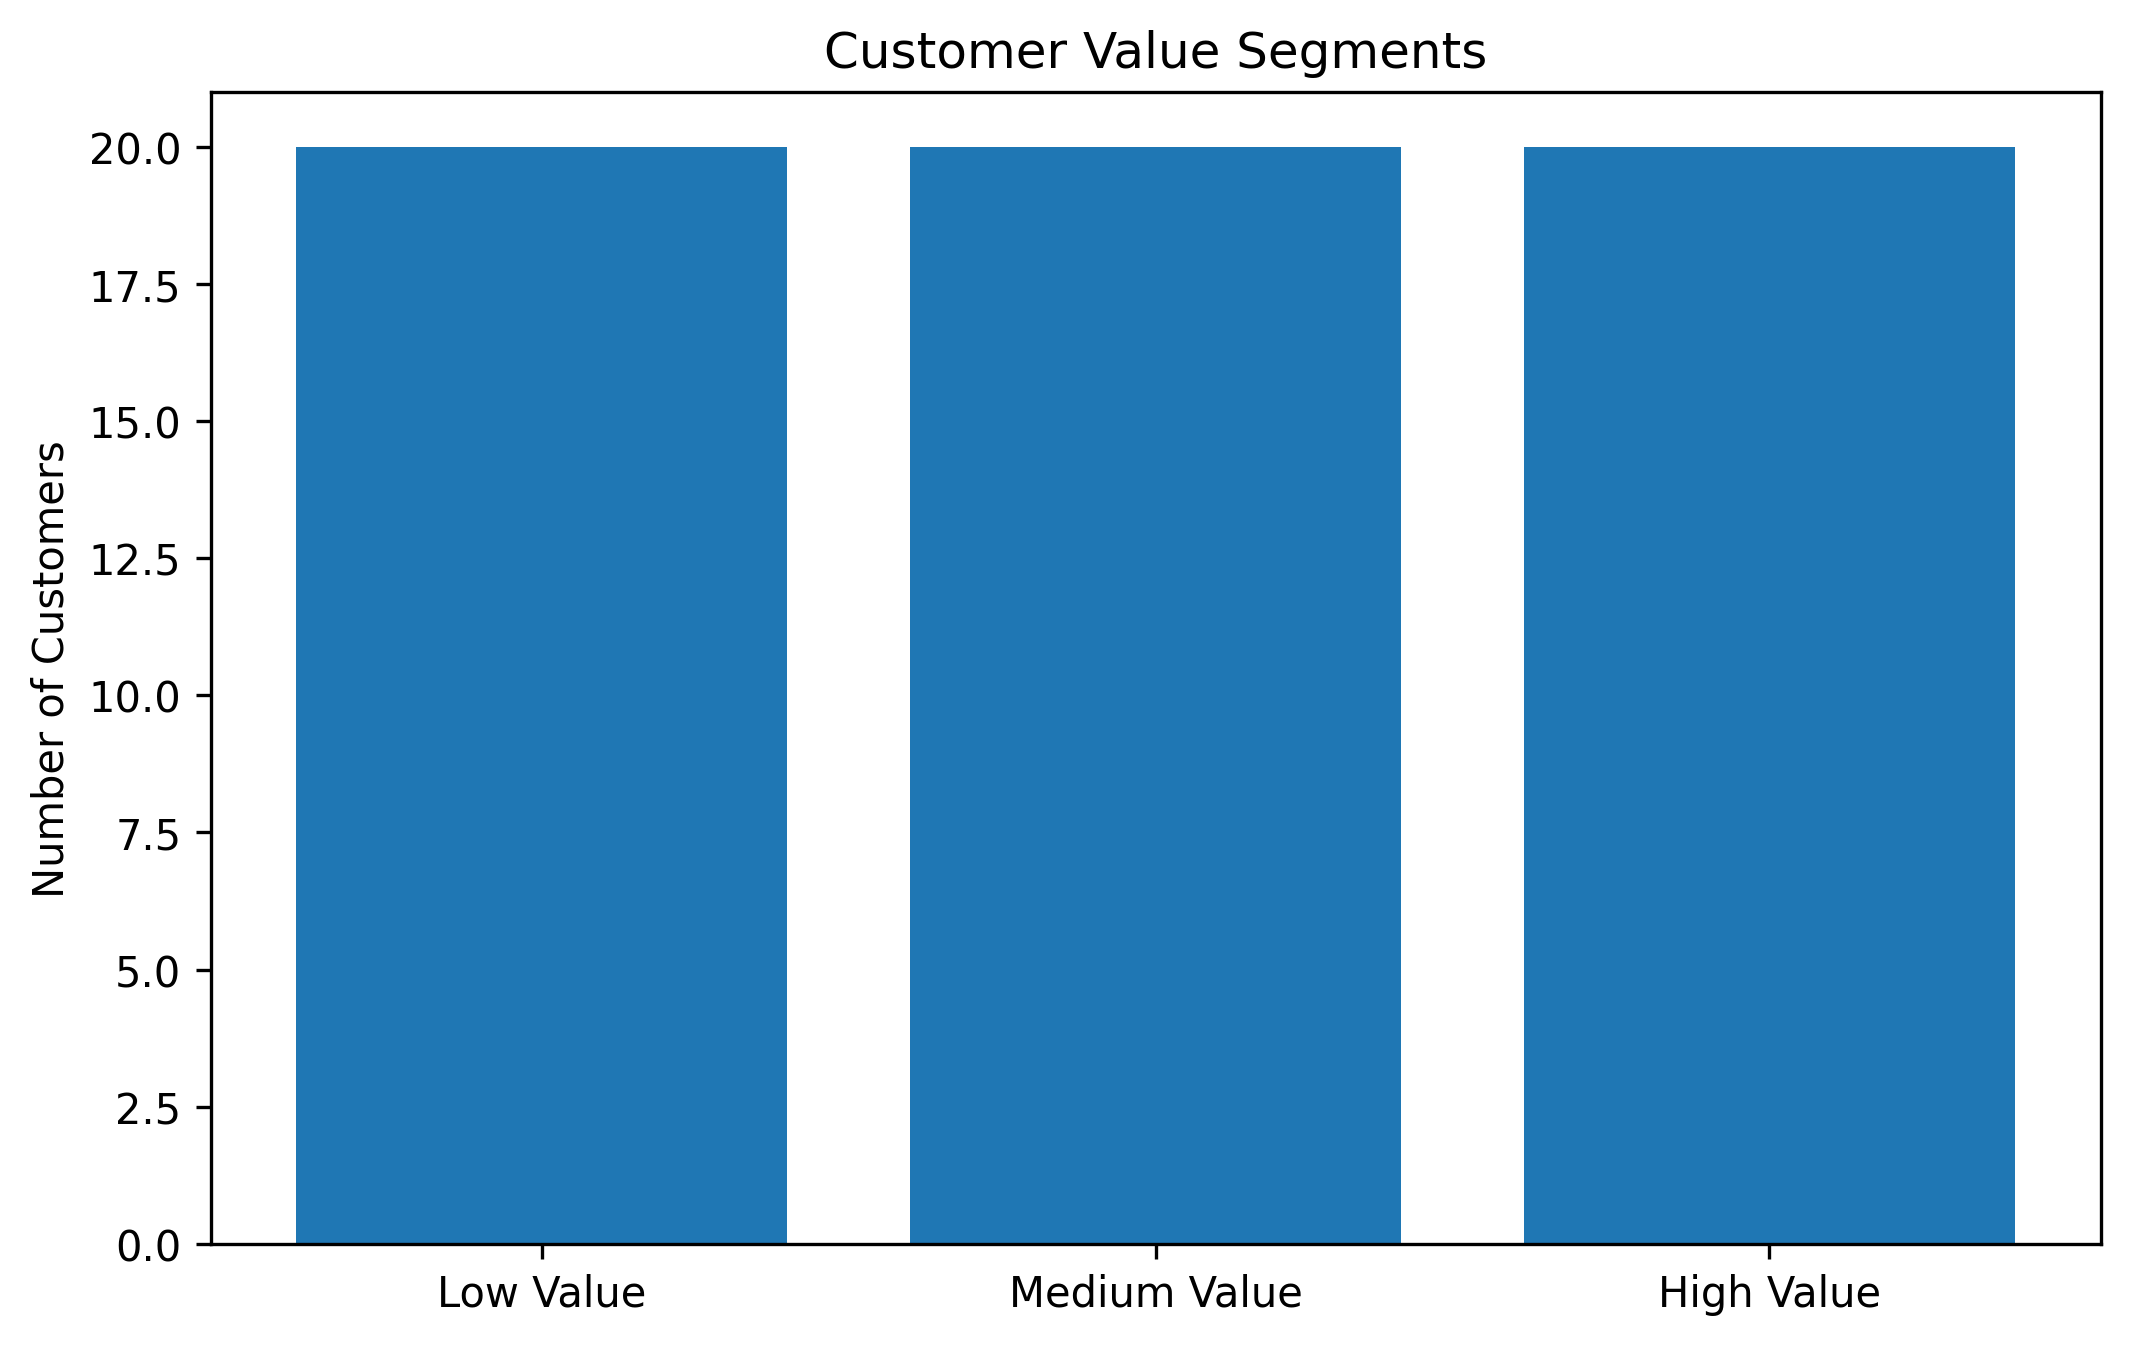
\includegraphics[width=0.82\textwidth]{fig02_customer_value_segments.png}
\caption{Customer-value segmentation reconstructed from the reported analytical output: 20 customers in each value group.}
\label{fig:value_segments}
\end{figure}


A composite Customer Value Score was developed using standardized versions of Total Spending, Purchase Count, and Average Order Value.

The score is defined as:

\[
CVS=
0.50Z(TS)
+
0.30Z(PC)
+
0.20Z(AOV),
\]

where:

\begin{itemize}
    \item $TS$ = Total Spending,
    \item $PC$ = Purchase Count,
    \item $AOV$ = Average Order Value.
\end{itemize}

Total Spending receives the largest weight because it represents realized customer revenue.

Customers were divided into three equal-sized value groups using empirical quantiles.

\begin{table}[H]
\centering
\caption{Customer value segments}
\label{tab:value_segments}
\begin{tabular}{lcc}
\toprule
\textbf{Segment} & \textbf{Customers} & \textbf{Share}\\
\midrule
Low Value & 20 & 33.3\%\\
Medium Value & 20 & 33.3\%\\
High Value & 20 & 33.3\%\\
\bottomrule
\end{tabular}
\end{table}

The segmentation provides a transparent basis for differentiated customer management.

% =========================================================
% 8 CHURN
% =========================================================

\section{Churn-Risk Analysis}

\begin{figure}[H]
\centering
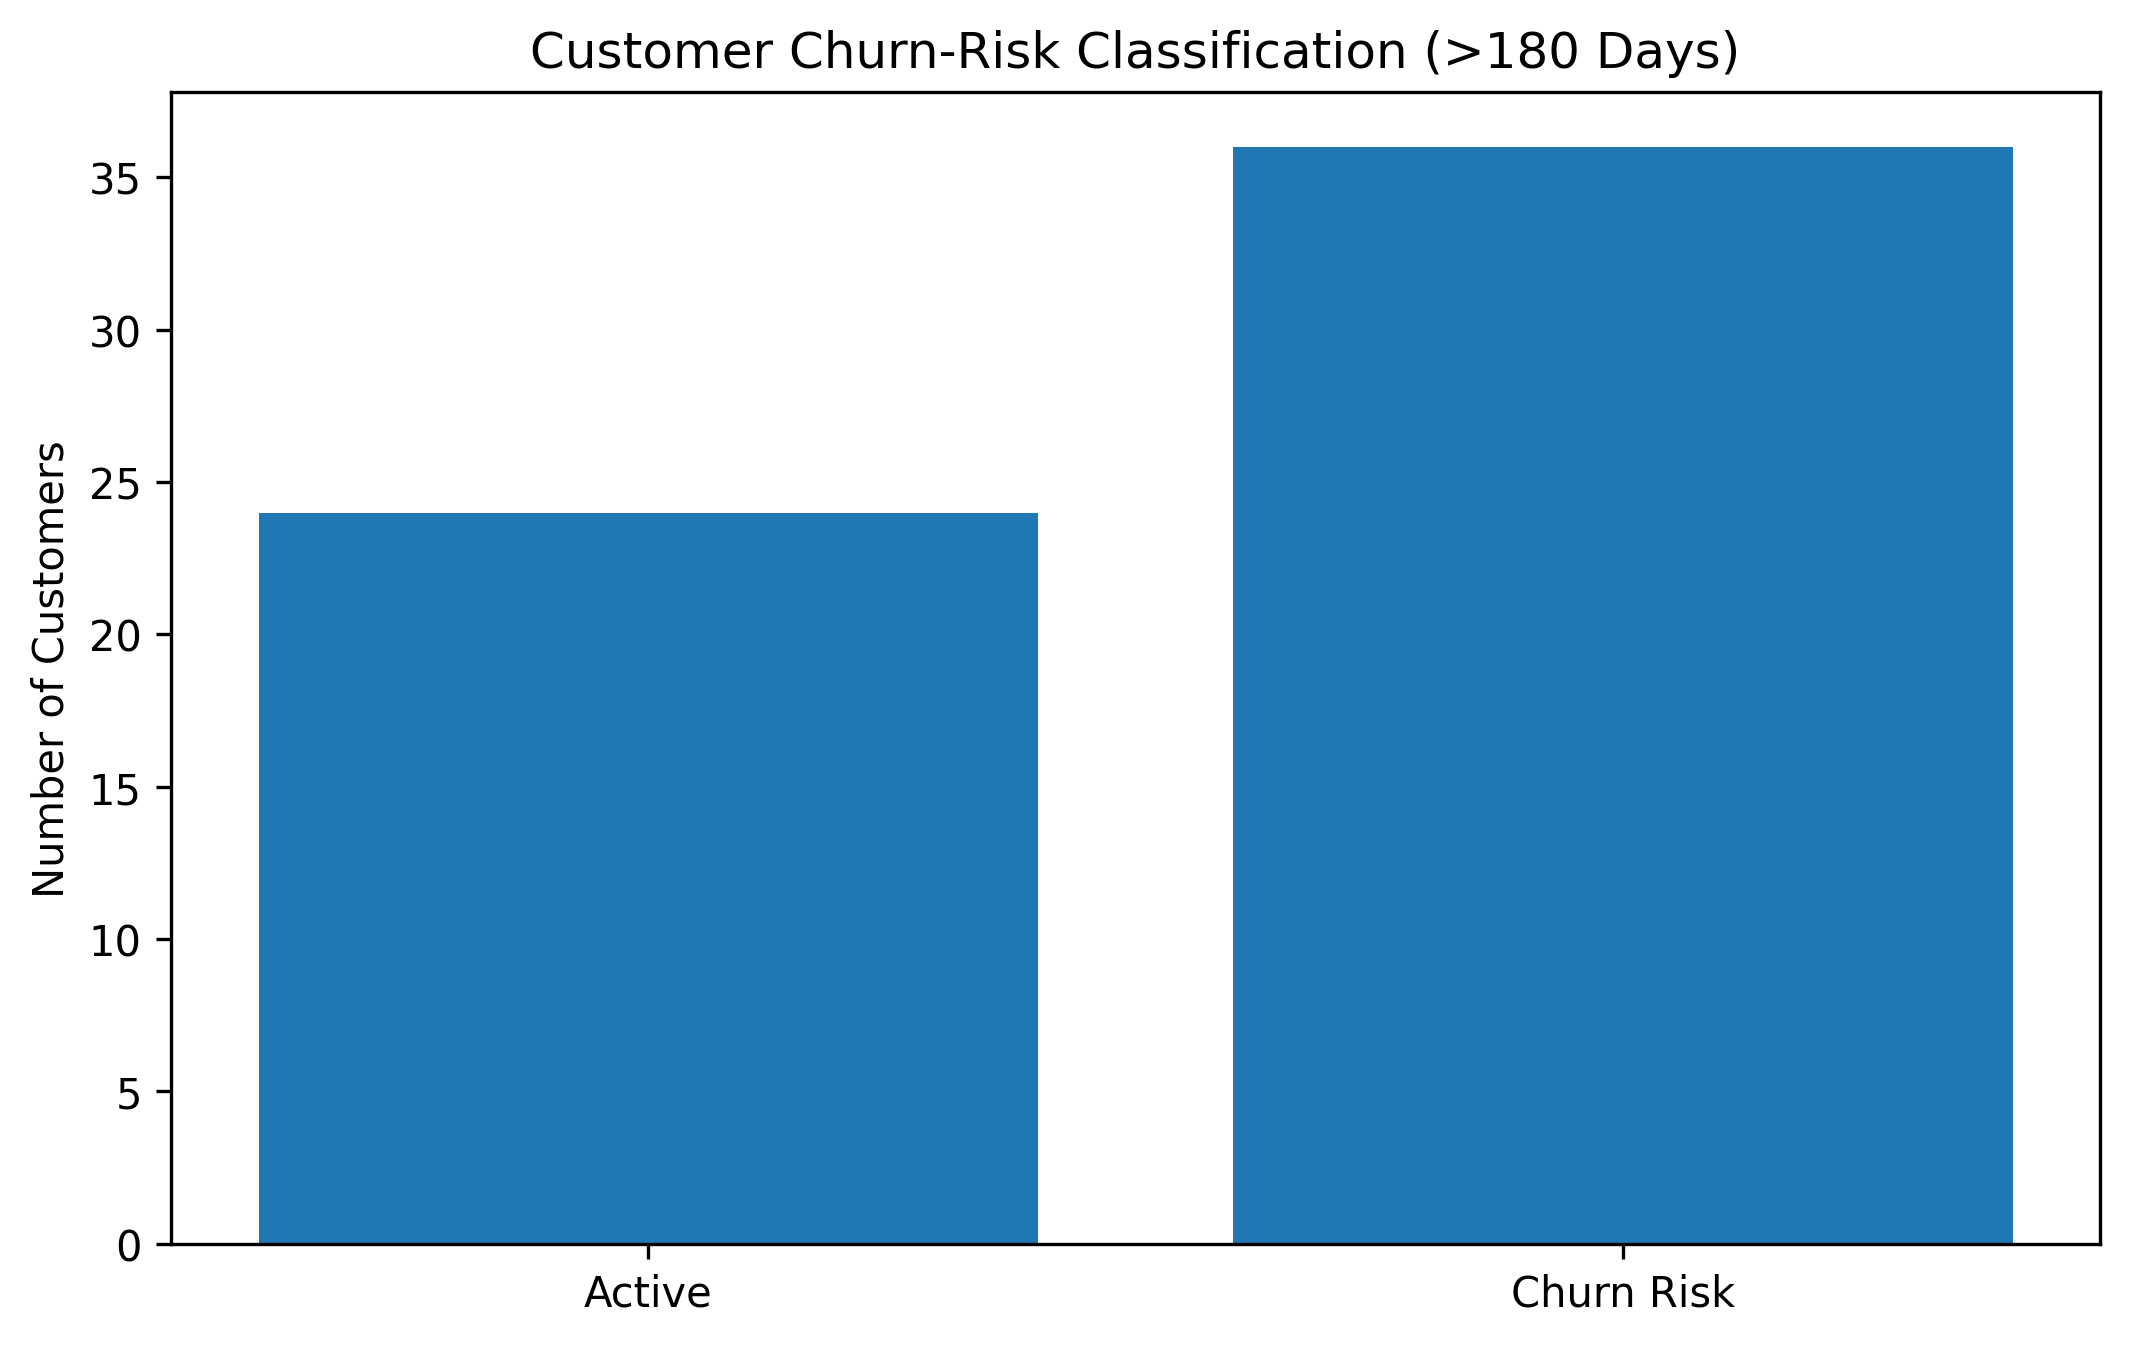
\includegraphics[width=0.78\textwidth]{fig03_churn_risk.png}
\caption{Operational churn-risk classification based on the 180-day inactivity threshold.}
\label{fig:churn_risk}
\end{figure}


Churn risk was operationalized using customer inactivity.

A customer was classified as churn-risk when:

\[
\text{Last Purchase Days}>180.
\]

The resulting classification is presented in Table~\ref{tab:churn}.

\begin{table}[H]
\centering
\caption{Churn-risk classification}
\label{tab:churn}
\begin{tabular}{lcc}
\toprule
\textbf{Status} & \textbf{Customers} & \textbf{Percentage}\\
\midrule
Active & 24 & 40\%\\
Churn Risk & 36 & 60\%\\
\bottomrule
\end{tabular}
\end{table}

Thus,

\[
\frac{36}{60}\times100=60\%.
\]

A particularly important group consists of customers who are both High Value and Churn Risk.

There are 12 such customers:

\[
\frac{12}{60}\times100=20\%.
\]

This group should receive the highest retention priority.

It is important to emphasize that churn is defined here as an inactivity-based proxy rather than an observed future churn outcome.

% =========================================================
% 9 KMEANS
% =========================================================

\section{Customer Segmentation Using K-Means}

\begin{figure}[H]
\centering
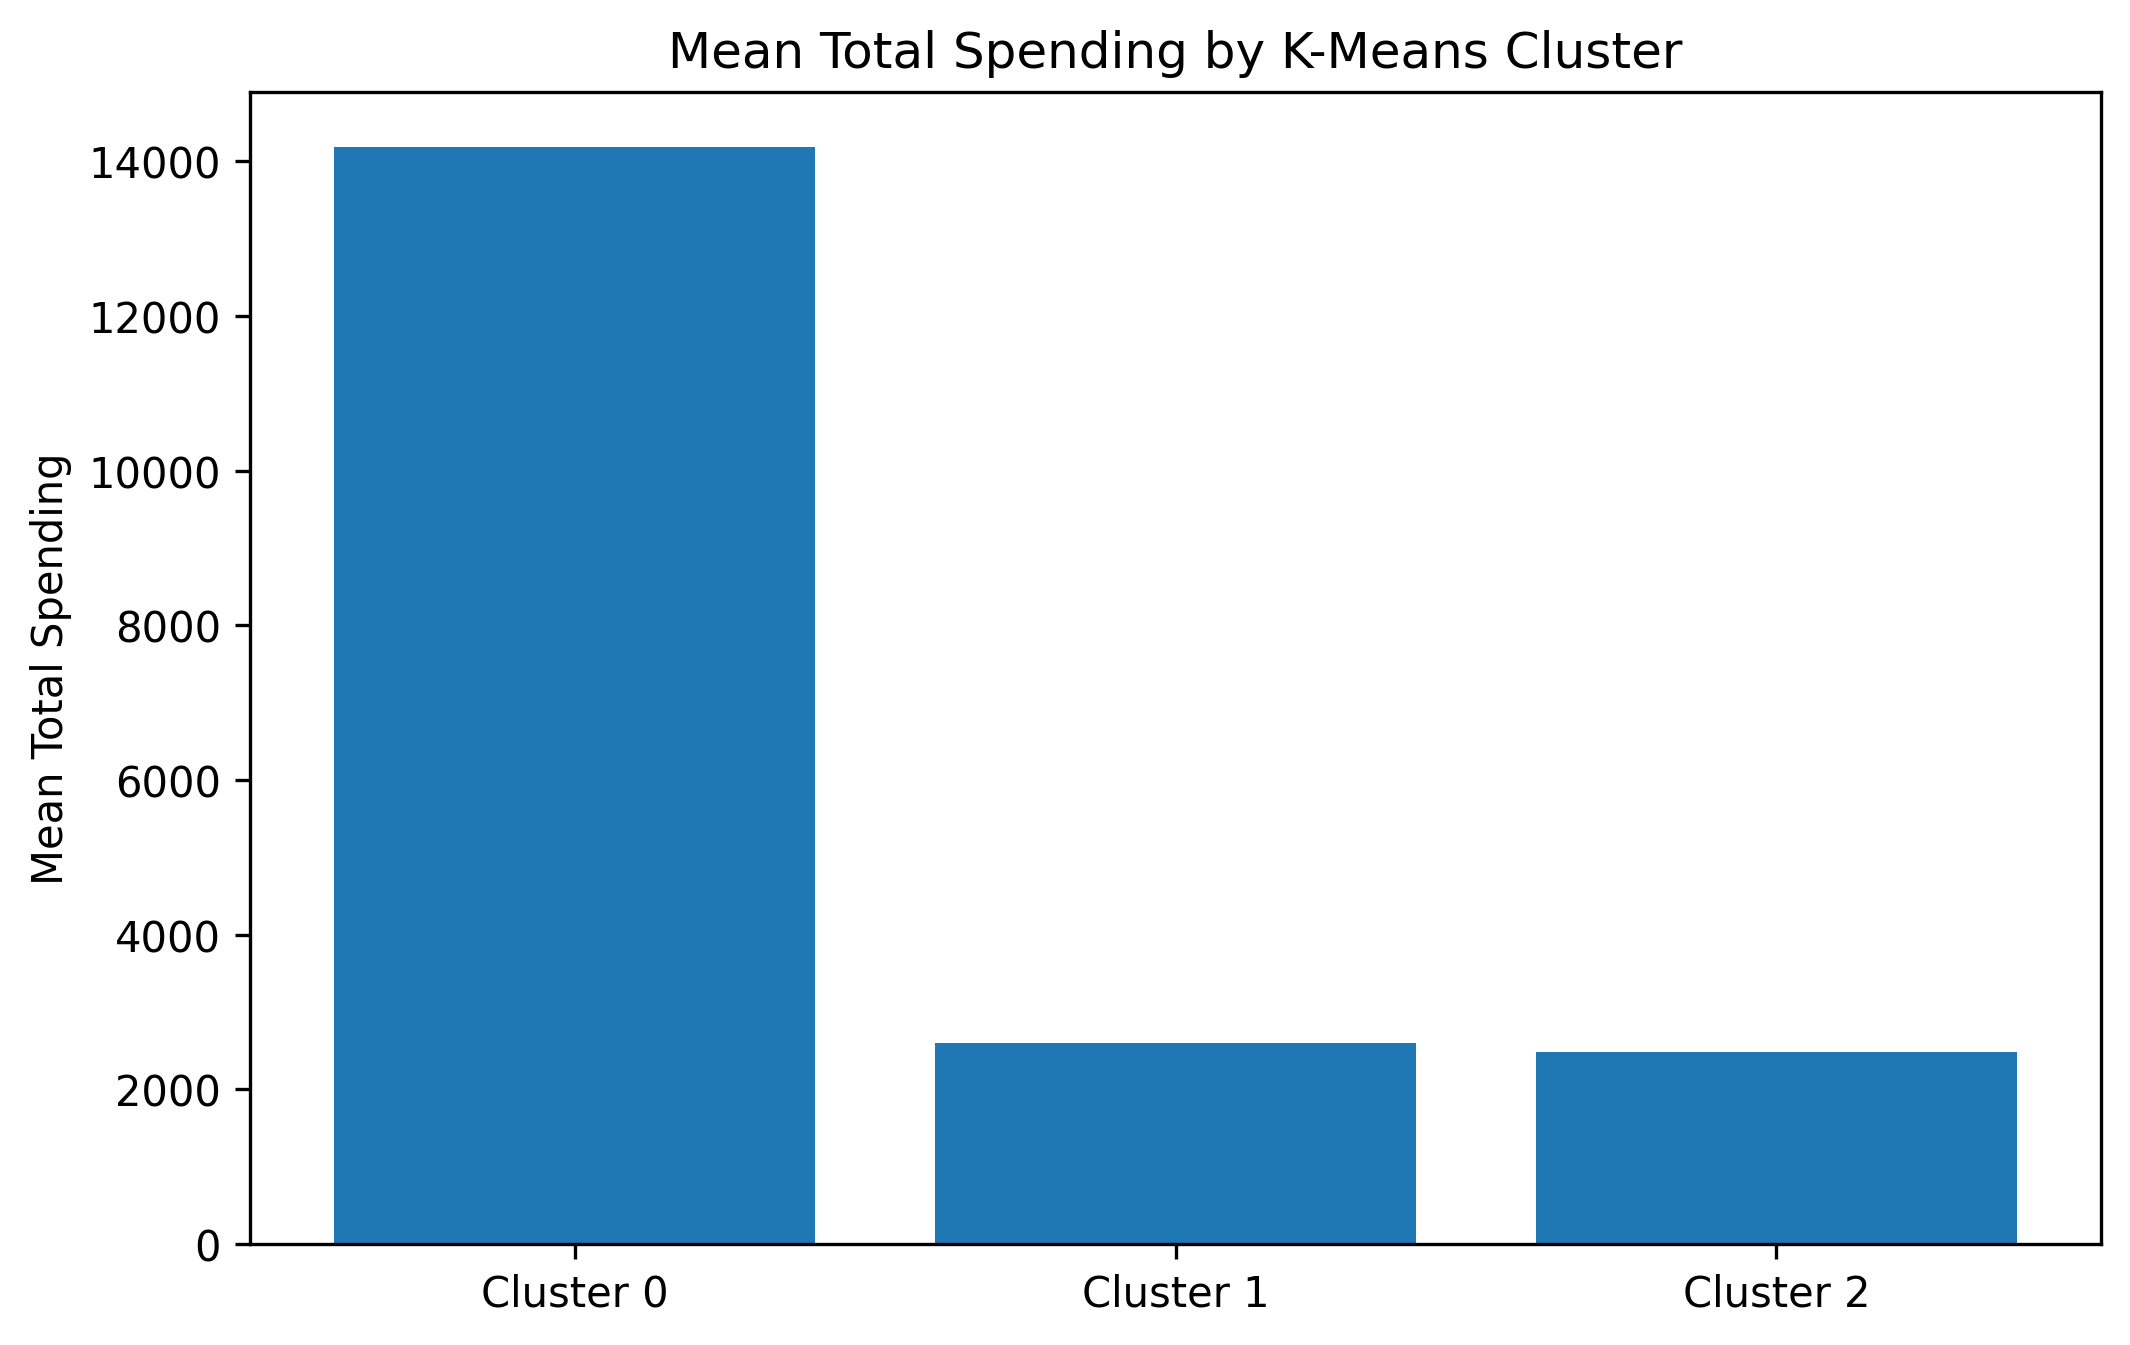
\includegraphics[width=0.82\textwidth]{fig06_customer_clusters.png}
\caption{Mean total spending across the three K-Means clusters, reconstructed from the reported cluster profiles.}
\label{fig:cluster_spending}
\end{figure}


K-Means clustering was applied using:

\begin{itemize}
    \item Purchase Count,
    \item Average Order Value,
    \item Total Spending,
    \item Last Purchase Days.
\end{itemize}

The variables were standardized before clustering.

The quality of candidate cluster solutions was assessed using the silhouette coefficient.

\begin{table}[H]
\centering
\caption{Silhouette scores for candidate cluster solutions}
\label{tab:silhouette}
\begin{tabular}{cc}
\toprule
\textbf{Number of Clusters} & \textbf{Silhouette Score}\\
\midrule
2 & 0.280\\
3 & \textbf{0.316}\\
4 & 0.297\\
5 & 0.308\\
6 & 0.299\\
\bottomrule
\end{tabular}
\end{table}

The highest silhouette score occurred at $K=3$.

Therefore, three clusters were selected.

% =========================================================
% 10 CLUSTER PROFILES
% =========================================================

\section{Cluster Profiles and Statistical Validation}

The three identified clusters are summarized in Table~\ref{tab:clusters}.

\begin{table}[H]
\centering
\caption{K-Means customer cluster profiles}
\label{tab:clusters}
\begin{adjustbox}{max width=\textwidth}
\begin{tabular}{lrrrrr}
\toprule
\textbf{Cluster} &
\textbf{Customers} &
\textbf{Avg. Purchases} &
\textbf{Avg. AOV} &
\textbf{Avg. Spending} &
\textbf{Avg. Inactivity}\\
\midrule
Cluster 0 & 6 & 30.33 & 348.60 & 14,188.76 & 211.17\\
Cluster 1 & 23 & 8.30 & 309.07 & 2,603.76 & 232.17\\
Cluster 2 & 31 & 21.61 & 115.78 & 2,475.26 & 173.81\\
\bottomrule
\end{tabular}
\end{adjustbox}
\end{table}

\subsection{Cluster 0: Premium Customers}

Cluster 0 contains only six customers but has an average total spending of approximately 14,188.76.

This cluster represents the company's most economically valuable behavioral group.

Recommended strategies include VIP retention, personalized communication, premium services, early access, and targeted relationship management.

\subsection{Cluster 1: Low-Frequency Customers}

Cluster 1 contains 23 customers with an average purchase count of 8.30 and average inactivity of approximately 232 days.

This group is suitable for reactivation strategies and personalized engagement.

\subsection{Cluster 2: Frequent Low-Basket Customers}

Cluster 2 contains 31 customers with relatively high purchase frequency but an average order value of only 115.78.

This segment provides a strong opportunity for cross-selling, bundling, and upselling.

\subsection{Kruskal--Wallis Validation}

To statistically evaluate whether total spending differs across clusters, the Kruskal--Wallis test was applied.

The test statistic was:

\[
H=16.109,
\]

with:

\[
p=0.000318.
\]

Since:

\[
p<0.05,
\]

the null hypothesis of identical spending distributions across the clusters is rejected.

Therefore, statistically significant differences in customer spending exist across the identified segments.

% =========================================================
% 11 MACHINE LEARNING
% =========================================================

\section{Machine-Learning Churn Analysis}

Two supervised learning algorithms were evaluated:

\begin{enumerate}
    \item Logistic Regression
    \item Random Forest
\end{enumerate}

Predictors included:

\begin{itemize}
    \item Age
    \item Purchase Count
    \item Average Order Value
    \item Total Spending
    \item Satisfaction Score
    \item Returned Items
\end{itemize}

The variable \texttt{last\_purchase\_days} was excluded because it directly defines the churn target. Including it would introduce target leakage.

\subsection{Cross-Validation Results}

Stratified five-fold cross-validation was used.

\begin{table}[H]
\centering
\caption{Cross-validated machine-learning performance}
\label{tab:ml}
\begin{tabular}{lcc}
\toprule
\textbf{Model} & \textbf{Mean ROC-AUC} & \textbf{Std. Dev.}\\
\midrule
Logistic Regression & \textbf{0.564} & 0.084\\
Random Forest & 0.478 & 0.096\\
\bottomrule
\end{tabular}
\end{table}

The results indicate weak predictive performance.

A ROC-AUC value near 0.50 corresponds approximately to random classification. Logistic Regression performs somewhat better than Random Forest, but neither model is sufficiently strong for production deployment.

% =========================================================
% 12 FEATURE IMPORTANCE
% =========================================================

\section{Random Forest Feature Importance}

\begin{figure}[H]
\centering
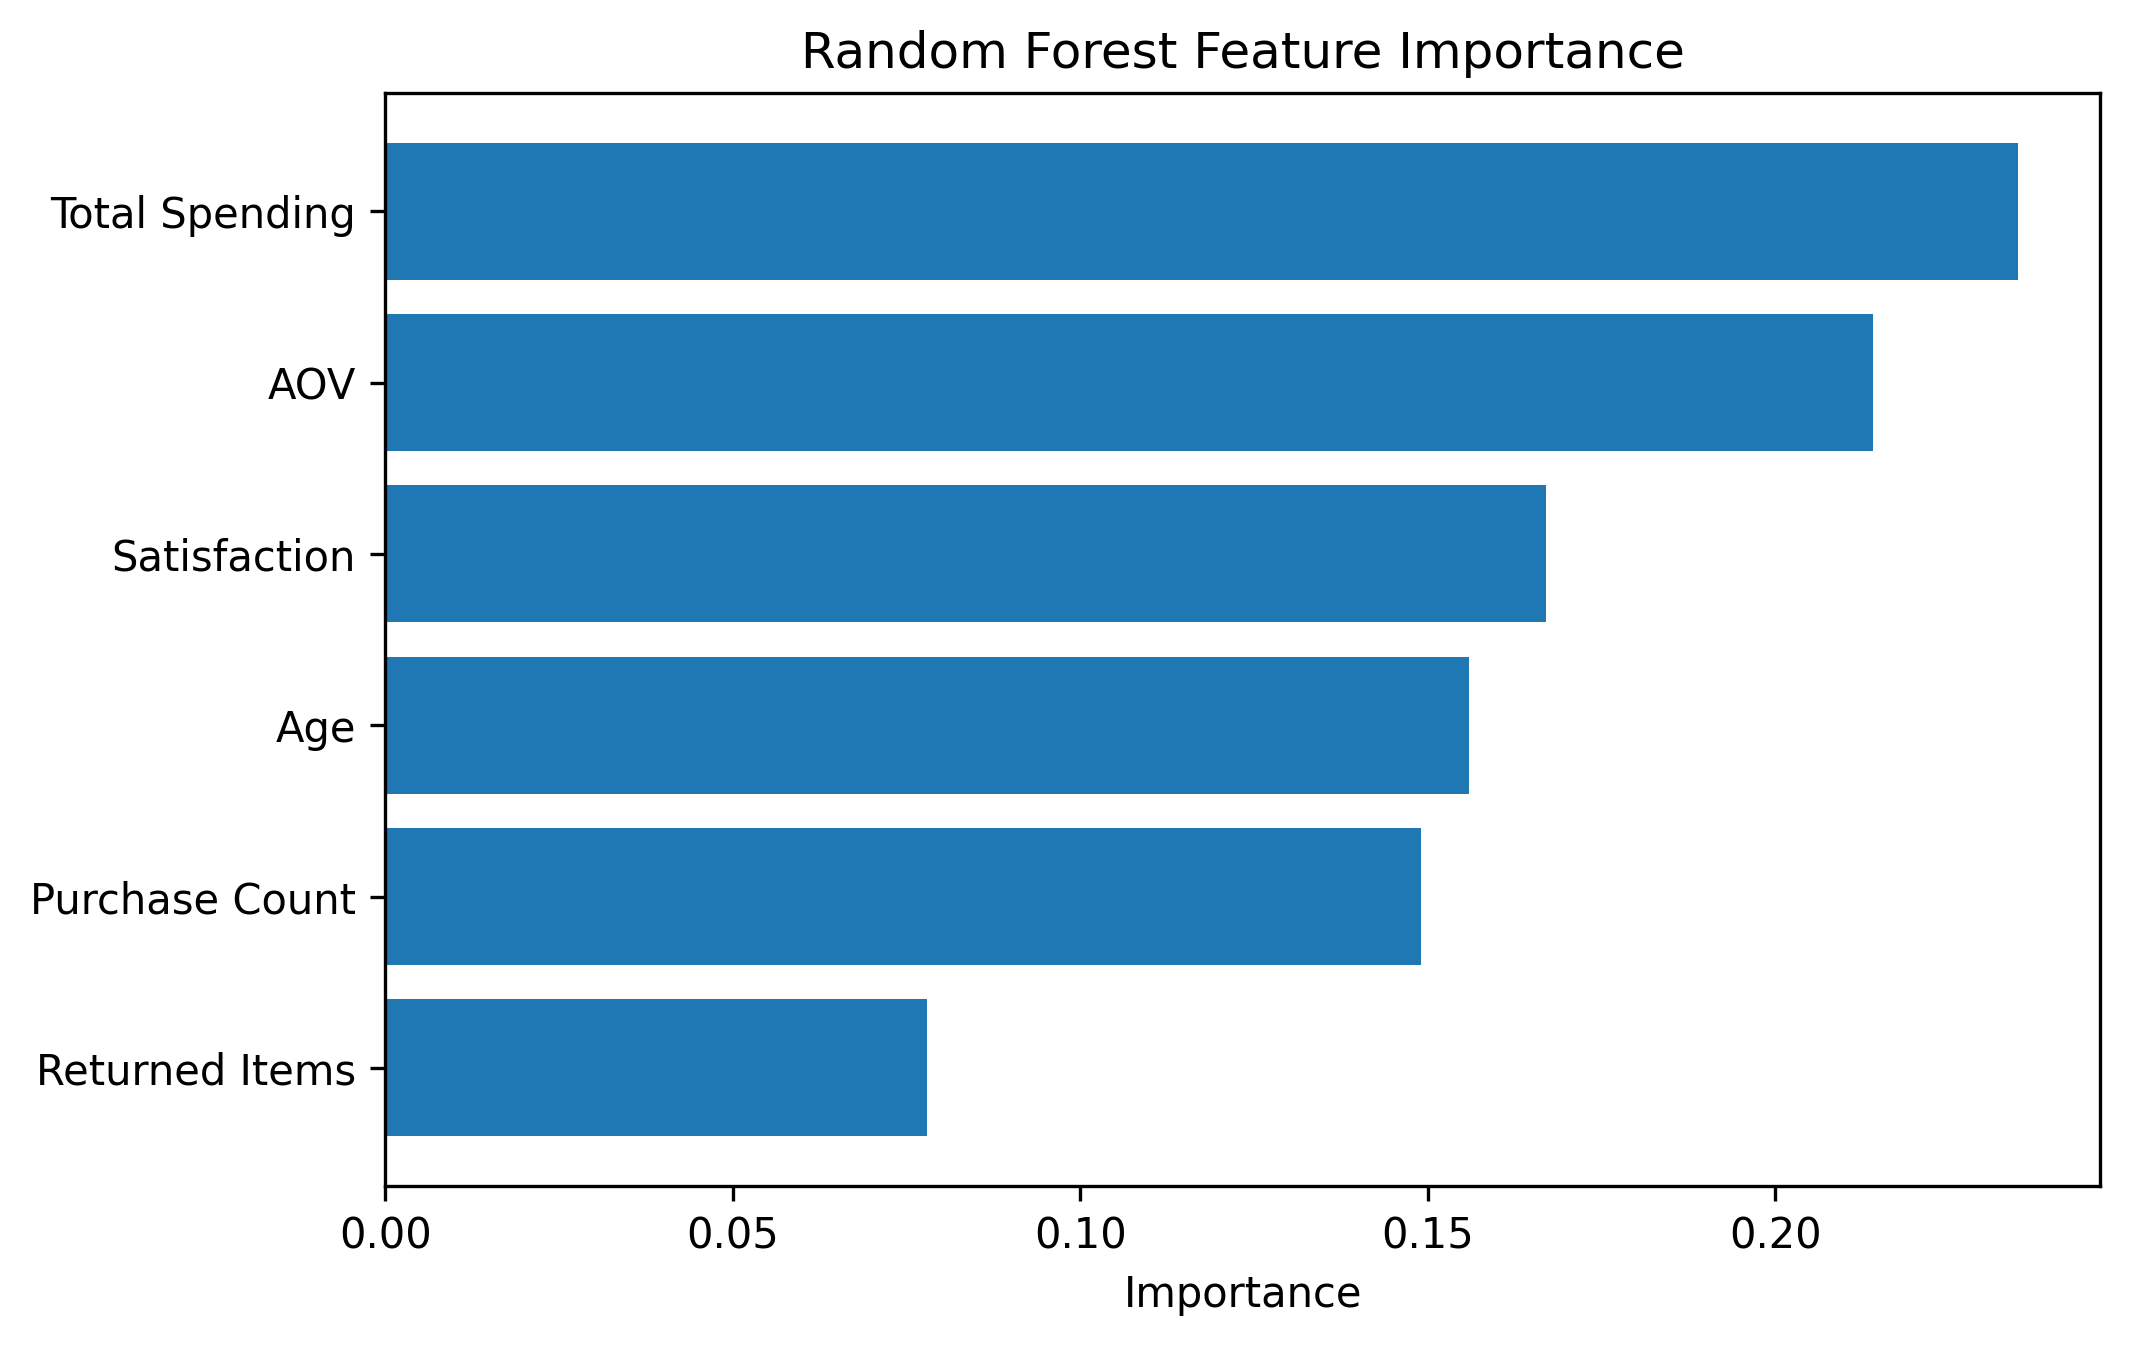
\includegraphics[width=0.82\textwidth]{fig09_random_forest_feature_importance.png}
\caption{Random Forest feature importance reconstructed from the reported model output.}
\label{fig:rf_importance}
\end{figure}


The estimated Random Forest feature importances are presented in Table~\ref{tab:importance}.

\begin{table}[H]
\centering
\caption{Random Forest feature importance}
\label{tab:importance}
\begin{tabular}{lr}
\toprule
\textbf{Feature} & \textbf{Importance}\\
\midrule
Total Spending & 0.235\\
Average Order Value & 0.214\\
Satisfaction Score & 0.167\\
Age & 0.156\\
Purchase Count & 0.149\\
Returned Items & 0.078\\
\bottomrule
\end{tabular}
\end{table}

Total Spending and Average Order Value were the two most influential variables within the fitted Random Forest.

These importance values should not be interpreted as causal effects.

% =========================================================
% 13 DISCOUNT
% =========================================================

\section{Discount Effectiveness Analysis}

\begin{figure}[H]
\centering
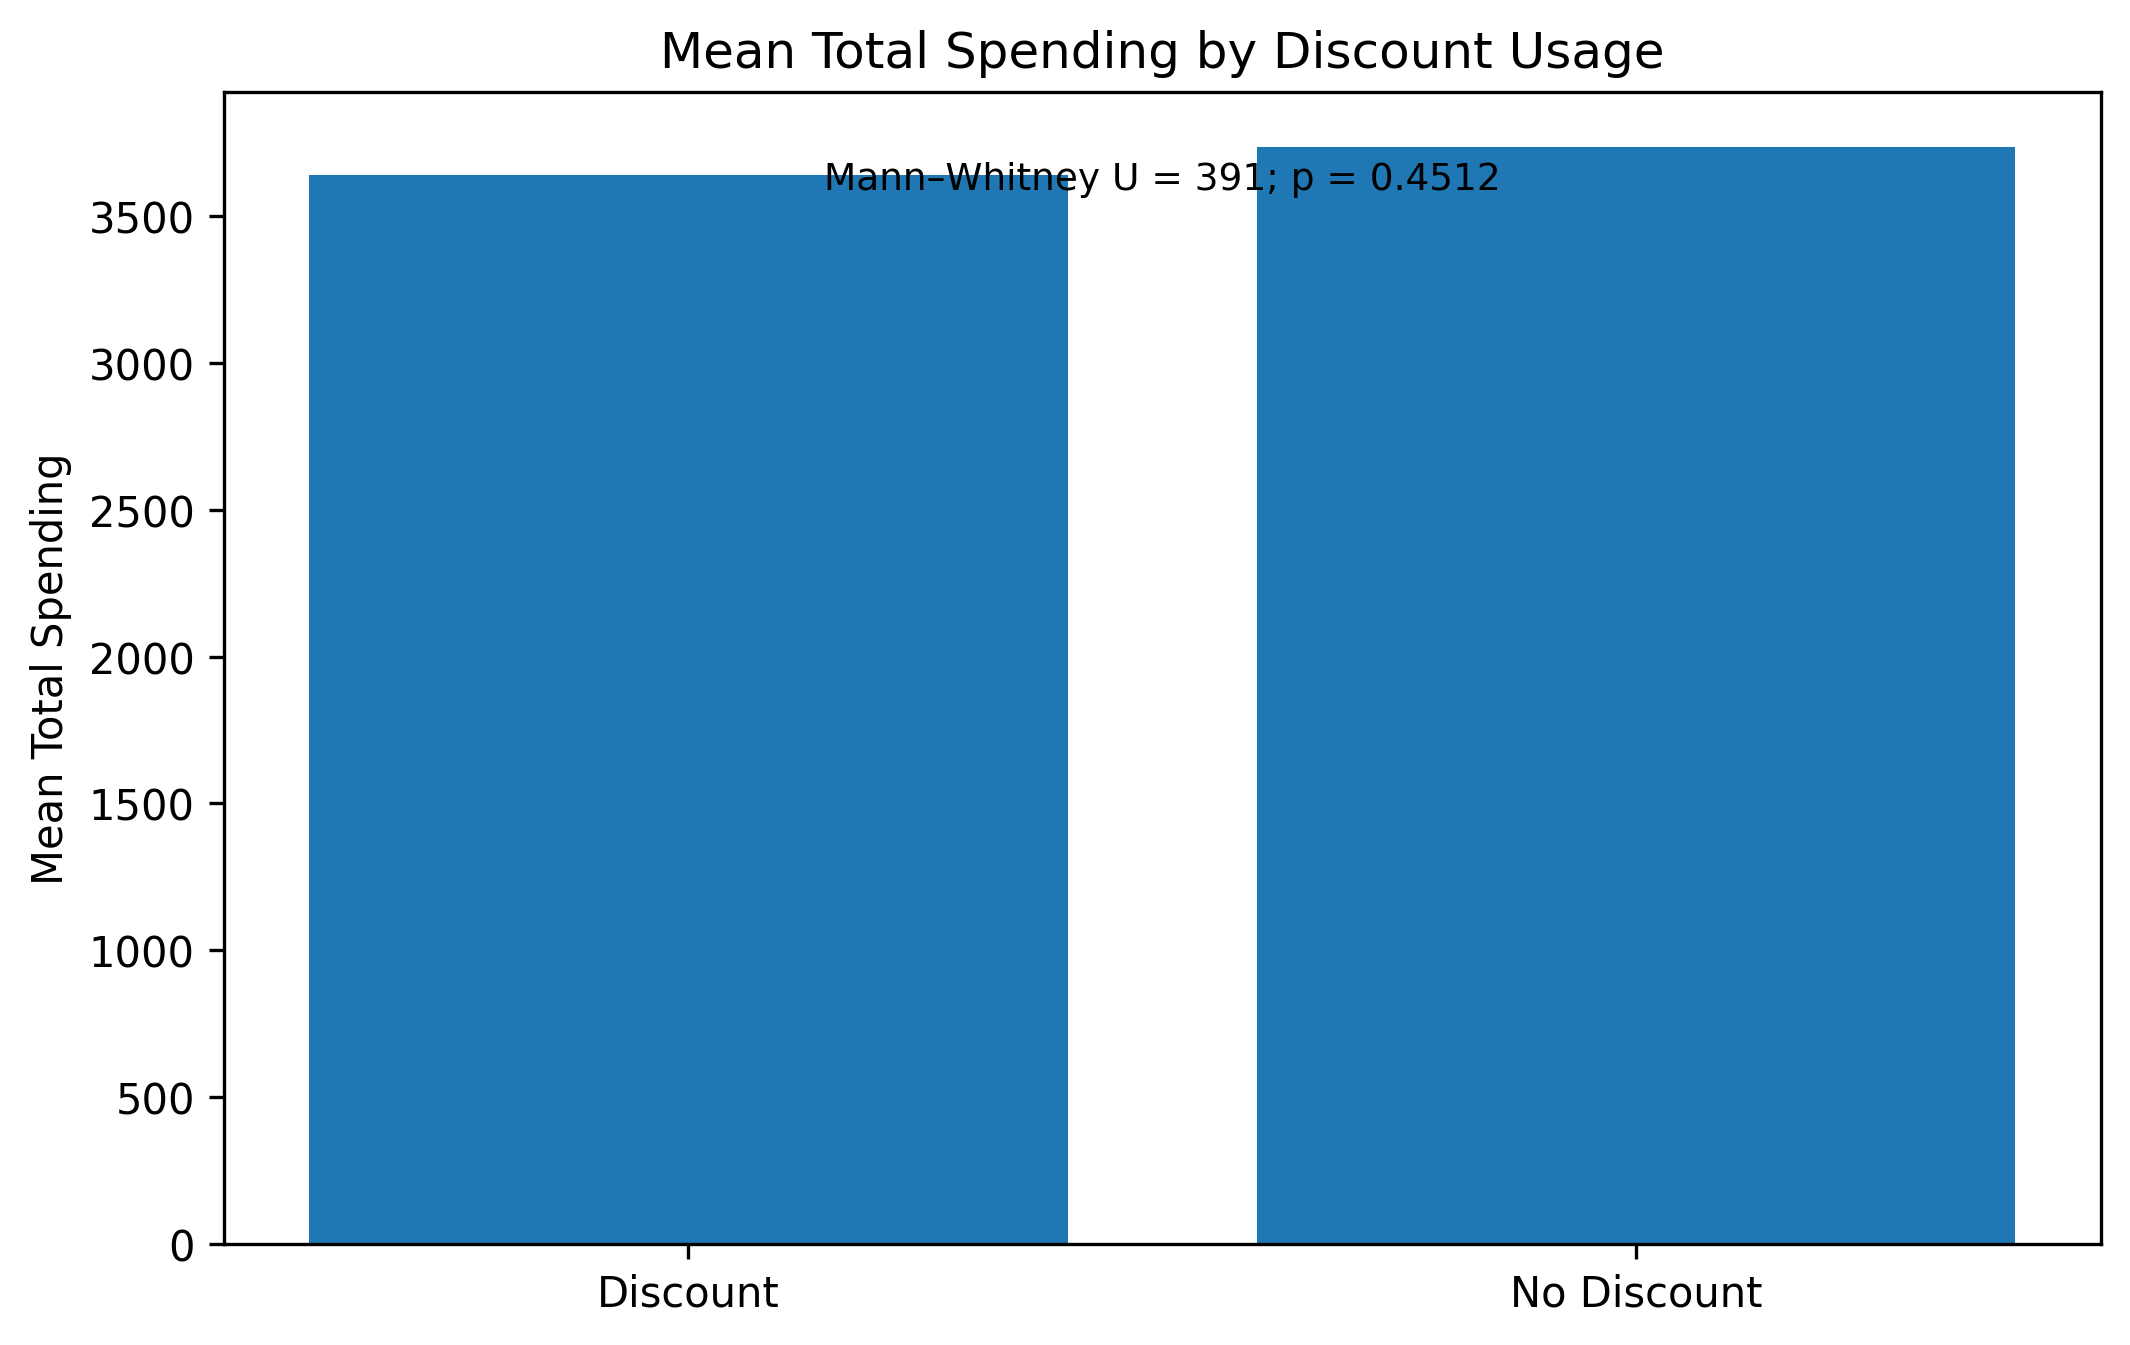
\includegraphics[width=0.78\textwidth]{fig07_discount_vs_spending.png}
\caption{Mean total spending by discount usage. The figure summarizes the reported group means and Mann--Whitney test result.}
\label{fig:discount_spending}
\end{figure}


Customers were divided into discount users and non-users.

\begin{table}[H]
\centering
\caption{Descriptive comparison of discount groups}
\label{tab:discount}
\begin{tabular}{lcc}
\toprule
\textbf{Metric} & \textbf{Discount} & \textbf{No Discount}\\
\midrule
Customers & 26 & 34\\
Mean Total Spending & 3,642.42 & 3,736.74\\
Mean AOV & 203.29 & 220.70\\
Mean Satisfaction & 3.27 & 2.76\\
\bottomrule
\end{tabular}
\end{table}

Because the data are non-normal, the Mann--Whitney U test was applied.

The results were:

\[
U=391,
\]

\[
p=0.4512.
\]

Since:

\[
p>0.05,
\]

there is no statistically significant evidence of a difference in total spending between the two groups.

The estimated Cohen's $d$ was approximately:

\[
d=-0.022.
\]

The bootstrap 95\% confidence interval for the mean spending difference was approximately:

\[
[-2146.19,\;2400.88].
\]

Because the confidence interval contains zero, the data do not provide strong evidence of a systematic spending difference.

Importantly, this does not demonstrate that discounts are ineffective. The observational design does not establish causality.

% =========================================================
% 14 CITY
% =========================================================

\section{City-Level Marketing Opportunity}

\begin{figure}[H]
\centering
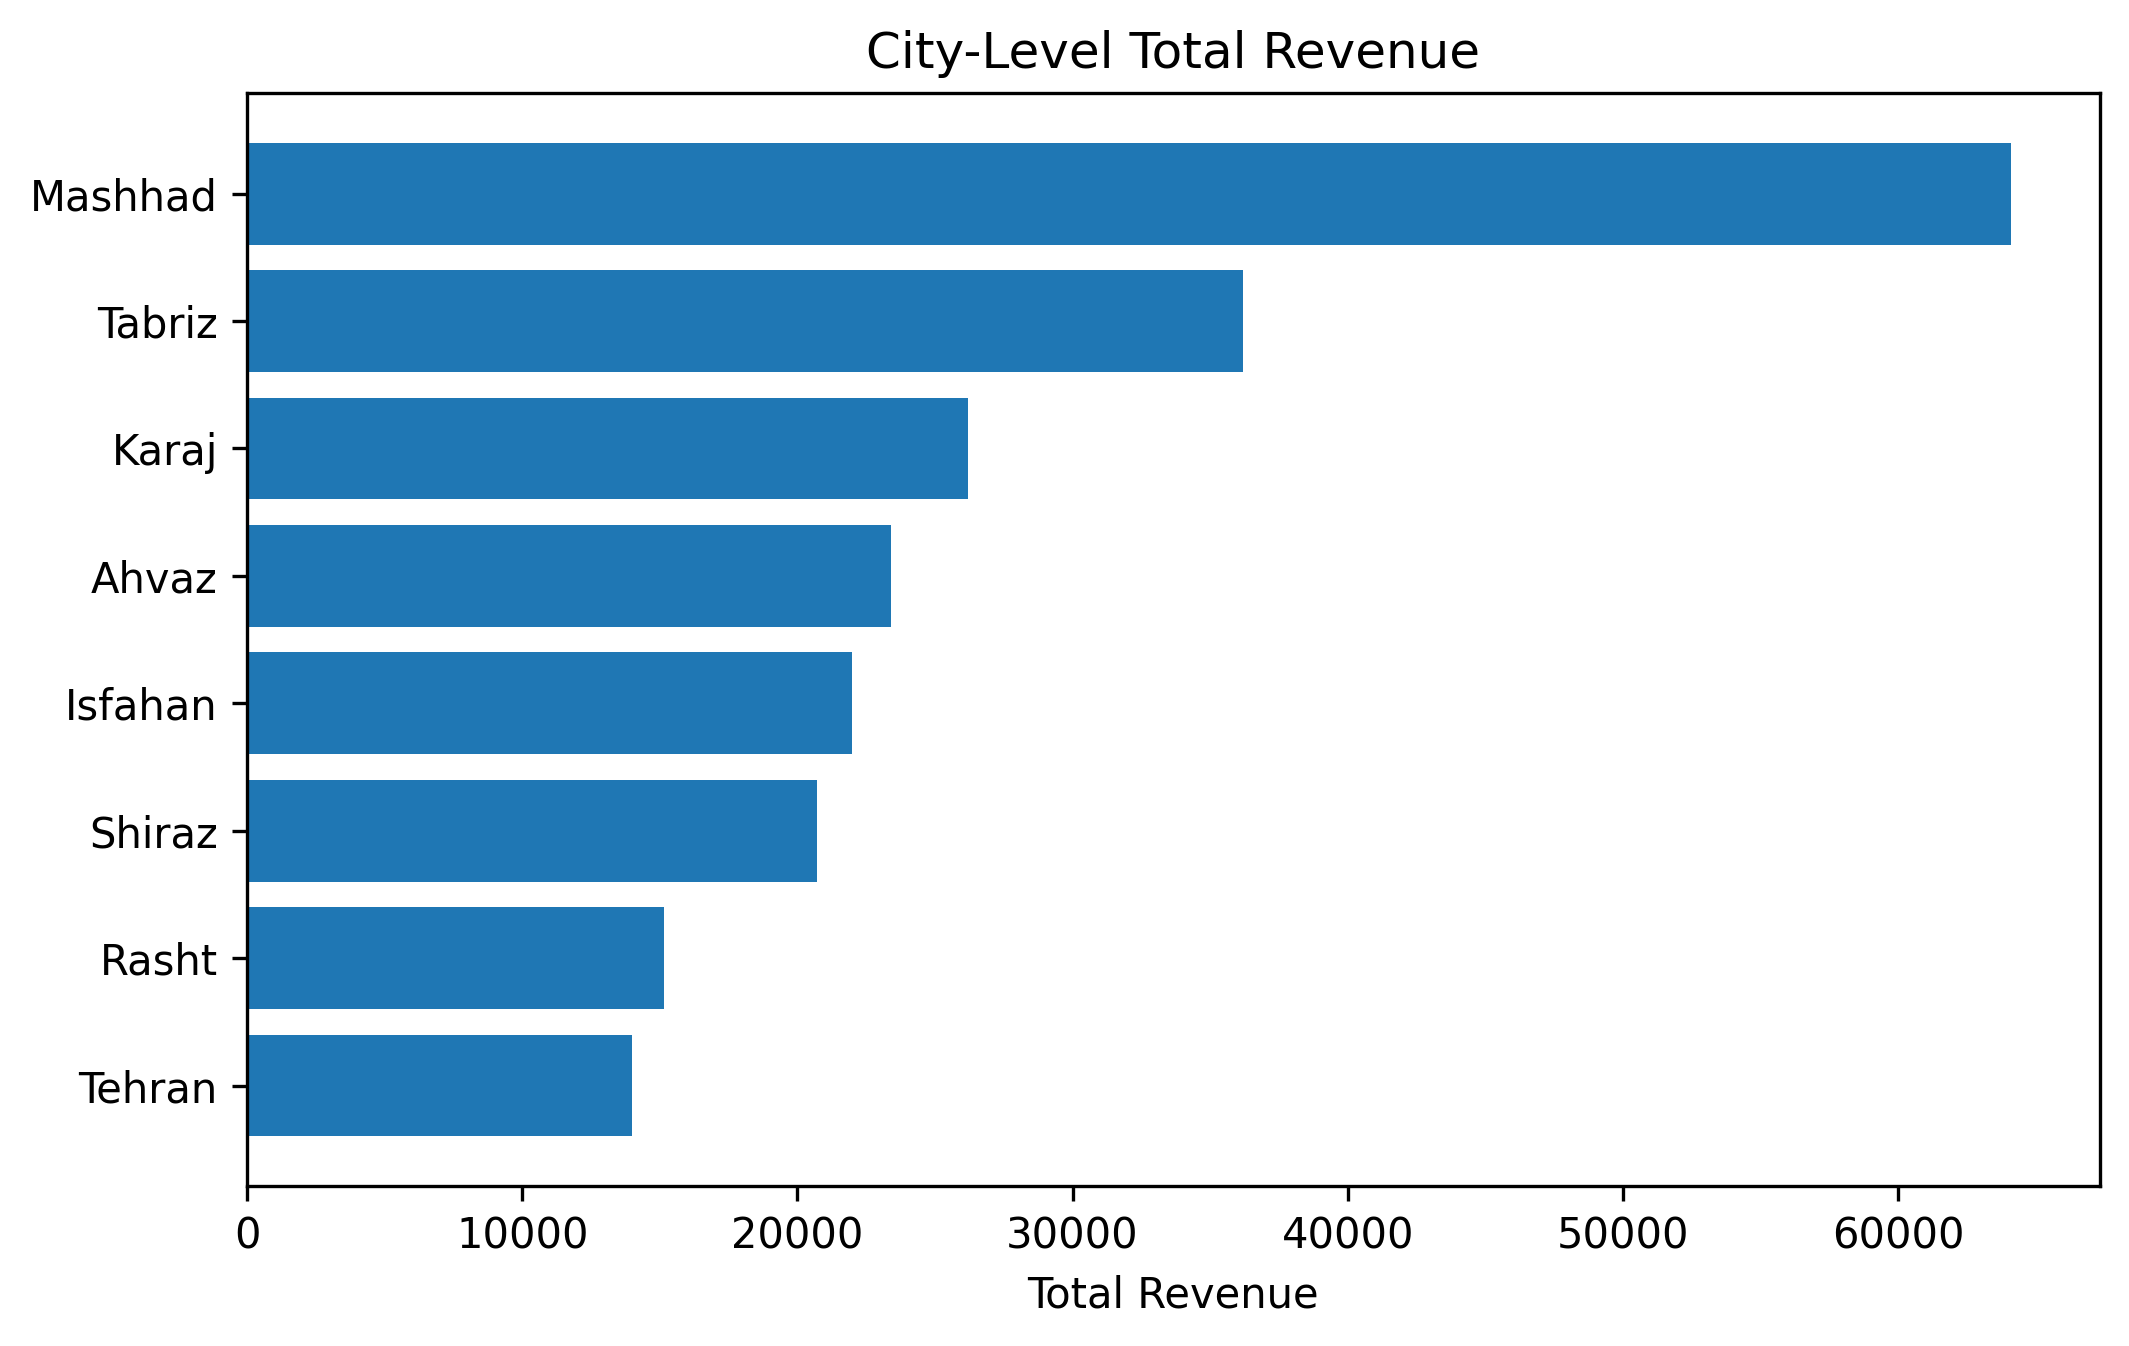
\includegraphics[width=0.86\textwidth]{fig08_city_revenue.png}
\caption{Observed total revenue by city. Mashhad has the highest reported total revenue.}
\label{fig:city_revenue}
\end{figure}


City-level marketing opportunity was evaluated using customer count, total revenue, average customer value, and satisfaction.

Table~\ref{tab:city} presents the principal city-level results.

\begin{table}[H]
\centering
\caption{Selected city-level customer and revenue indicators}
\label{tab:city}
\begin{adjustbox}{max width=\textwidth}
\begin{tabular}{lrrrr}
\toprule
\textbf{City} &
\textbf{Customers} &
\textbf{Total Revenue} &
\textbf{Avg. Spending} &
\textbf{Avg. Satisfaction}\\
\midrule
Mashhad & 11 & 64,118.44 & 5,828.95 & 2.91\\
Tabriz & 12 & 36,192.49 & 3,016.04 & 3.00\\
Karaj & 7 & 26,189.81 & 3,741.40 & 2.86\\
Ahvaz & 8 & 23,384.78 & 2,923.10 & 3.50\\
Isfahan & 5 & 21,975.32 & 4,395.06 & 4.40\\
Shiraz & 6 & 20,715.92 & 3,452.65 & 2.00\\
Rasht & 5 & 15,168.54 & 3,033.71 & 2.60\\
Tehran & 6 & 14,006.85 & 2,334.48 & 2.67\\
\bottomrule
\end{tabular}
\end{adjustbox}
\end{table}

Mashhad achieved the highest observed total revenue:

\[
R_{\text{Mashhad}}=64,118.44.
\]

It also recorded the highest average customer spending among the listed cities.

Therefore, Mashhad represents the strongest candidate for a controlled marketing experiment.

However, the average satisfaction score of 2.91 indicates that customer-experience problems should be investigated before aggressively scaling acquisition.

% =========================================================
% 15 BUSINESS RECOMMENDATIONS
% =========================================================

\section{Membership and Channel Analysis}

Membership tiers exhibited heterogeneous economic profiles. Gold
customers generated the highest total revenue, 75,153.20, while Silver
customers had the highest mean spending per customer, approximately
4,179.93. VIP customers had a higher mean satisfaction score of 3.40,
whereas Silver customers had the lowest satisfaction score at 2.50.

Payment-channel analysis showed that cash payments generated the largest
total revenue (80,781.87), followed by online wallet payments (71,402.63)
and card payments (69,567.65).

Device analysis showed that web users generated approximately 78,876.06
in revenue, followed by Android users at 74,945.08 and iPhone users at
67,931.01. These figures describe observed channel performance and should
not be interpreted causally without controlling for customer composition
and exposure.

% =========================================================

\section{Age and Satisfaction Profiles}

The 55+ age group exhibited the highest mean spending, approximately
6,592.10, and an average purchase count of 21.35. Younger age groups
generally exhibited lower spending levels.

The relationship between satisfaction and spending was not monotonic
enough to support a simple linear interpretation. Customers with a
satisfaction score of 4 had mean spending of approximately 5,448.63,
whereas the score-5 group had mean spending of approximately 2,677.52.

This pattern demonstrates why customer satisfaction should not be treated
as a direct proxy for economic value. Satisfaction and spending represent
different dimensions of customer behavior and should be modeled jointly.

% =========================================================

\section{Integrated Statistical Interpretation}

The statistical evidence supports four broad conclusions.

First, customer value is highly concentrated. The high-value segment
contains only one-third of customers but generates approximately 70.77\%
of revenue. This concentration increases the economic importance of
retention among high-value customers.

Second, the customer base exhibits substantial behavioral heterogeneity.
The non-normal distributions, moderate correlations, and significant
cluster differences all indicate that a single average customer profile
would be an inadequate representation of the population.

Third, churn risk is operationally substantial. Sixty percent of the
sample meets the selected recency-based risk criterion, and 12 customers
combine high economic value with elevated recency risk. These customers
should be prioritized before broad, undifferentiated retention campaigns.

Fourth, the evidence does not support universal discounting as a reliable
revenue-growth mechanism. The Mann--Whitney test, near-zero effect size,
and bootstrap confidence interval are all consistent with the conclusion
that discount usage did not produce a detectable general spending
difference in this sample.

% =========================================================

\section{Business Recommendations}

The analytical results lead to three principal recommendations.

\subsection{Recommendation 1: High-Value Customer Retention}

The company should immediately prioritize the 12 customers who are both High Value and Churn Risk.

Potential actions include:

\begin{itemize}
    \item Personalized communication
    \item VIP benefits
    \item Exclusive product recommendations
    \item Early product access
    \item Personalized incentives
    \item Customer-service follow-up
\end{itemize}

The main performance indicators should include:

\begin{itemize}
    \item Reactivation Rate
    \item Revenue Recovered
    \item Repeat Purchase Rate
    \item Customer Lifetime Value
    \item Cost per Reactivated Customer
\end{itemize}

\subsection{Recommendation 2: Increase Average Order Value}

The 31 customers in Cluster 2 represent a major upselling opportunity.

Recommended tactics include:

\begin{itemize}
    \item Product bundles
    \item Cross-selling
    \item Complementary-product recommendations
    \item Free-shipping thresholds
    \item Quantity-based offers
    \item Premium-product recommendations
\end{itemize}

The primary KPI should be Average Order Value.

\subsection{Recommendation 3: Controlled Marketing Experiment in Mashhad}

Mashhad should be considered for a controlled marketing pilot.

A randomized experimental design is recommended:

\begin{center}
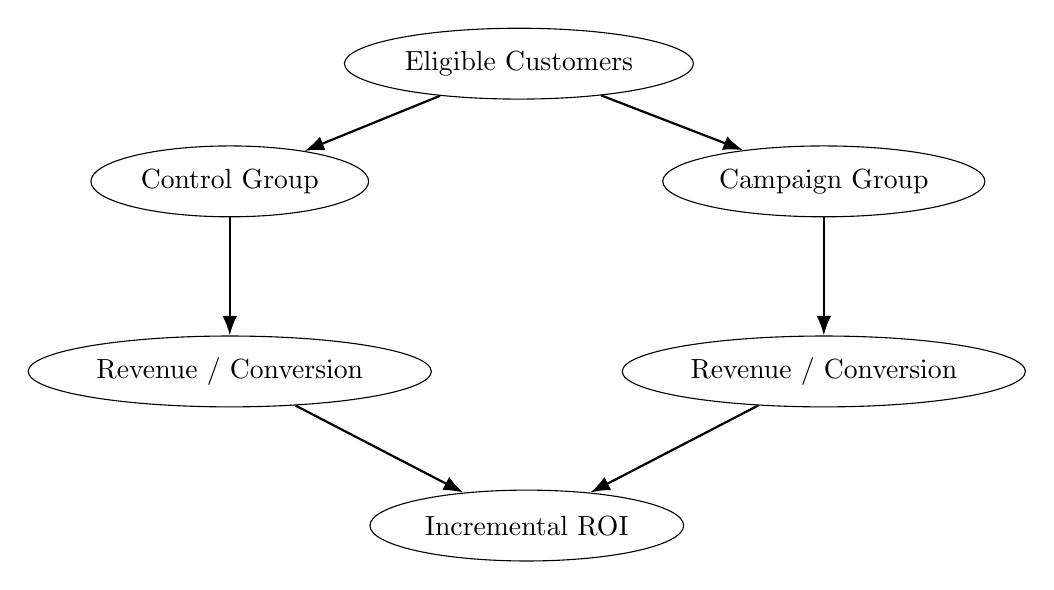
\begin{tikzpicture}[
node distance=1.2cm,
process/.style={
    draw,
    ellipse,
    minimum width=3.5cm,
    minimum height=0.9cm,
    align=center
},
arrow/.style={-{Latex[length=2.5mm]}, thick}
]

\node[process] (customers) {Eligible Customers};
\node[process, below left=of customers] (control) {Control Group};
\node[process, below right=of customers] (treat) {Campaign Group};
\node[process, below=1.5cm of control] (cresult) {Revenue / Conversion};
\node[process, below=1.5cm of treat] (tresult) {Revenue / Conversion};
\node[process, below=1.5cm of $(cresult)!0.5!(tresult)$] (decision) {Incremental ROI};

\draw[arrow] (customers) -- (control);
\draw[arrow] (customers) -- (treat);
\draw[arrow] (control) -- (cresult);
\draw[arrow] (treat) -- (tresult);
\draw[arrow] (cresult) -- (decision);
\draw[arrow] (tresult) -- (decision);

\end{tikzpicture}
\end{center}

The experiment should evaluate incremental revenue, conversion, repeat purchasing, customer satisfaction, and Return on Advertising Spend (ROAS).

% =========================================================
% 16 STRATEGY MATRIX
% =========================================================

\section{Customer Strategy Matrix}

\begin{table}[H]
\centering
\caption{Recommended customer-management strategies}
\label{tab:strategy}
\begin{adjustbox}{max width=\textwidth}
\begin{tabular}{p{3.3cm}p{4cm}p{5cm}}
\toprule
\textbf{Customer Type} &
\textbf{Main Problem} &
\textbf{Recommended Action}\\
\midrule
High Value + Churn Risk &
Risk of losing high revenue &
Immediate personalized retention\\

High Value + Active &
Protect existing value &
VIP loyalty and relationship management\\

Frequent + Low AOV &
Low basket size &
Upselling and cross-selling\\

Low Frequency + Churn Risk &
Low engagement &
Reactivation campaign\\

Discount Users &
Unclear incremental value &
Targeted A/B-tested discounts\\

Mashhad Customers &
High commercial opportunity &
Controlled marketing experiment\\
\bottomrule
\end{tabular}
\end{adjustbox}
\end{table}

% =========================================================
% 17 LIMITATIONS
% =========================================================


\subsection{Figure Provenance}
\label{subsec:figure_provenance}

The empirical figures in this article are based exclusively on numerical
results reported by the project's analytical workflow and source report.
Where the original PNG outputs were not available as standalone files in
the current file set, the corresponding figures were reconstructed from
the reported numerical outputs without introducing new observations.


\section{Limitations}

\subsection{Small Sample Size}

The dataset contains only 60 customers. Consequently, machine-learning estimates may be unstable and should be considered exploratory.

\subsection{Proxy Churn Definition}

Churn was defined using:

\[
\text{Last Purchase Days}>180.
\]

This is a business-rule proxy rather than an observed future churn event.

\subsection{Observational Discount Analysis}

Customers were not randomly assigned to discount and non-discount groups. Therefore, causal conclusions about discount effectiveness cannot be established.

\subsection{Potential Sampling Bias}

The available customer sample may not represent the complete customer population.

\subsection{Machine-Learning Performance}

The Logistic Regression model achieved a mean ROC-AUC of approximately 0.564, while Random Forest achieved approximately 0.478.

These results do not justify production deployment.

% =========================================================
% 18 FUTURE RESEARCH
% =========================================================

\section{Future Research}

A production-level customer analytics system should incorporate longitudinal transaction data.

Important additional variables include:

\begin{itemize}
    \item Transaction timestamps
    \item Product identifiers
    \item Product categories
    \item Quantity
    \item Price
    \item Discount amount
    \item Gross revenue
    \item Profit margin
    \item Website sessions
    \item App activity
    \item Cart abandonment
    \item Email engagement
    \item Campaign exposure
\end{itemize}

A genuine churn target should be defined as a future behavioral outcome.

For example:

\[
Y_i=
\begin{cases}
1, & \text{if customer }i\text{ does not purchase during the future window},\\
0, & \text{otherwise}.
\end{cases}
\]

A temporal train-test split should then be used to estimate true out-of-time predictive performance.

Potential future algorithms include:

\begin{itemize}
    \item Logistic Regression
    \item Random Forest
    \item Gradient Boosting
    \item XGBoost
    \item Survival Analysis
\end{itemize}

Performance should be evaluated using ROC-AUC, Precision-Recall AUC (PR-AUC), calibration, and business-cost metrics.

% =========================================================
% 19 CONCLUSION
% =========================================================

\section{Overall Conclusion}

This study demonstrates how customer-level data can be transformed into actionable business intelligence through an integrated statistical and machine-learning framework.

The analysis revealed substantial heterogeneity in customer value. Twenty customers were classified as High Value, while K-Means clustering identified a particularly valuable behavioral segment containing only six customers with an average total spending of approximately 14,188.76.

The churn-risk analysis identified 36 inactive customers, representing 60\% of the sample under the selected inactivity rule. More importantly, 12 customers were simultaneously classified as High Value and Churn Risk. These customers represent the most strategically important retention group.

The K-Means segmentation was supported by the Kruskal--Wallis test, which produced:

\[
H=16.109,\qquad p=0.000318.
\]

Thus, customer spending differs significantly across the identified behavioral segments.

The discount analysis did not detect a statistically significant spending difference:

\[
U=391,\qquad p=0.4512.
\]

Consequently, broad discounting cannot be justified based solely on the current observational evidence. Controlled experiments are recommended to estimate the incremental effect of discounts.

At the geographical level, Mashhad achieved the highest observed total revenue of approximately 64,118.44. However, its moderate satisfaction level indicates that marketing expansion should be accompanied by improvements in customer experience.

The machine-learning results were limited. Logistic Regression achieved a mean cross-validated ROC-AUC of approximately 0.564, whereas Random Forest achieved 0.478. These findings indicate that the current dataset is not sufficiently large or longitudinal for reliable production churn prediction.

Overall, the evidence supports a differentiated customer strategy rather than a one-size-fits-all marketing approach.

The recommended priority is therefore:

\[
\boxed{
\text{Protect High-Value Customers}
\rightarrow
\text{Increase AOV}
\rightarrow
\text{Validate Marketing Through Experiments}
}
\]

This framework provides a practical foundation for future customer analytics systems once larger and longitudinal datasets become available.

% =========================================================
% 20 MANAGEMENT ACTION PLAN
% =========================================================

This study demonstrates how SQL-based customer analytics can be extended
into a statistically grounded decision-support framework. The analysis
of 60 customers revealed pronounced heterogeneity in purchasing behavior,
customer value, geographic performance, and churn risk.

The strongest finding is the concentration of economic value: the
high-value third of the customer base accounts for approximately 70.77\%
of total revenue. At the same time, 36 customers, representing 60\% of
the sample, satisfy the operational churn-risk criterion. The intersection
of these two dimensions identifies 12 high-value customers who are also
at risk of churn. From a managerial perspective, this group represents
the most immediate retention opportunity because the potential economic
cost of losing these customers is substantially greater than that of
losing low-value customers.

The inferential analysis further shows that customer behavior cannot be
adequately summarized by simple means or normal-theory assumptions.
Several variables are significantly non-normal, motivating the use of
Spearman correlation, Mann--Whitney U, and Kruskal--Wallis procedures.
The clustering analysis identifies three statistically distinguishable
customer profiles, while the weak predictive AUC values indicate that
the current feature set is insufficient for reliable individual-level
churn prediction.

The discount analysis is particularly important for managerial
decision-making. No statistically significant spending difference was
detected between discount users and non-users ($p=0.4512$), the estimated
effect size was negligible, and the bootstrap confidence interval
contained zero. Consequently, discounts should be viewed as a tactical
instrument requiring targeting and experimentation rather than as a
general-purpose mechanism for increasing customer spending.

Finally, Mashhad emerged as the strongest revenue market, but its
moderate satisfaction level highlights the need to balance acquisition
with customer-experience improvement. Overall, the evidence supports a
data-driven strategy centered on value-based segmentation, targeted
retention, selective incentives, geographic prioritization, and stronger
data-quality controls. Future research should extend the analysis with
transaction-level temporal data, survival analysis, causal experiments
for discount effectiveness, and richer behavioral features to improve
predictive customer analytics.

% =========================================================

\section{Final Management Action Plan}

\begin{table}[H]
\centering
\caption{Prioritized management action plan}
\label{tab:action_plan}
\begin{adjustbox}{max width=\textwidth}
\begin{tabular}{clll}
\toprule
\textbf{Priority} &
\textbf{Action} &
\textbf{Target} &
\textbf{Primary KPI}\\
\midrule
1 &
High-value retention &
12 High Value + Churn Risk &
Reactivation Rate\\

2 &
Upselling and cross-selling &
31 frequent low-AOV customers &
Average Order Value\\

3 &
Marketing pilot &
Mashhad &
Incremental Revenue / ROI\\

4 &
Discount A/B testing &
Selected customer groups &
Revenue Lift\\

5 &
Improve churn data &
All customers &
Future ROC-AUC / PR-AUC\\
\bottomrule
\end{tabular}
\end{adjustbox}
\end{table}

The principal managerial conclusion is that customer resources should be allocated according to economic value, behavioral characteristics, and risk rather than treating all customers identically.

% =========================================================
% REFERENCES
% =========================================================

\section{Key Statistical Indicators}

\begin{table}[H]
\centering
\caption{Summary of principal analytical indicators}
\begin{tabular}{lr}
\toprule
Indicator & Value \\
\midrule
Sample size & 60 customers \\
Total revenue & 221,752.15 \\
Mean customer spending & 3,695.87 \\
Mean AOV & 213.16 \\
High-value customers & 20 \\
High-value revenue share & 70.77\% \\
Churn-risk customers & 36 (60\%) \\
High-value and churn-risk customers & 12 \\
Best city by total revenue & Mashhad \\
Mashhad total revenue & 64,118.44 \\
Mashhad mean spending & 5,828.95 \\
Discount test: Mann--Whitney $p$ & 0.4512 \\
Discount effect size: Cohen's $d$ & $\approx -0.022$ \\
Discount mean-difference bootstrap 95\% CI & $[-2146.19,2400.88]$ \\
Optimal K-means $k$ & 3 \\
Silhouette score & 0.316 \\
Kruskal--Wallis $H$ & 16.109 \\
Kruskal--Wallis $p$ & 0.000318 \\
Logistic Regression mean ROC-AUC & 0.564 \\
Random Forest mean ROC-AUC & 0.478 \\
\bottomrule
\end{tabular}
\end{table}

\begin{thebibliography}{99}

\bibitem{scikit}
F. Pedregosa, G. Varoquaux, A. Gramfort, et al.,
``Scikit-learn: Machine Learning in Python,''
\textit{Journal of Machine Learning Research}, vol. 12, pp. 2825--2830, 2011.

\bibitem{spearman}
C. Spearman,
``The proof and measurement of association between two things,''
\textit{The American Journal of Psychology}, vol. 15, no. 1, pp. 72--101, 1904.

\bibitem{kmeans}
J. MacQueen,
``Some methods for classification and analysis of multivariate observations,''
in \textit{Proceedings of the Fifth Berkeley Symposium on Mathematical Statistics and Probability}, pp. 281--297, University of California Press, 1967.

\bibitem{silhouette}
P. J. Rousseeuw,
``Silhouettes: A graphical aid to the interpretation and validation of cluster analysis,''
\textit{Journal of Computational and Applied Mathematics}, vol. 20, pp. 53--65, 1987.

\bibitem{mannwhitney}
H. B. Mann and D. R. Whitney,
``On a test of whether one of two random variables is stochastically larger than the other,''
\textit{The Annals of Mathematical Statistics}, vol. 18, no. 1, pp. 50--60, 1947.

\bibitem{shapiro}
S. S. Shapiro and M. B. Wilk,
``An analysis of variance test for normality (complete samples),''
\textit{Biometrika}, vol. 52, no. 3--4, pp. 591--611, 1965.

\bibitem{kruskal}
W. H. Kruskal and W. A. Wallis,
``Use of ranks in one-criterion variance analysis,''
\textit{Journal of the American Statistical Association}, vol. 47, no. 260, pp. 583--621, 1952.

\bibitem{cohen}
J. Cohen,
\textit{Statistical Power Analysis for the Behavioral Sciences}, 2nd ed., Lawrence Erlbaum Associates, 1988.

\bibitem{efron}
B. Efron and R. J. Tibshirani,
\textit{An Introduction to the Bootstrap}, Chapman \& Hall, 1993.

\bibitem{breiman}
L. Breiman,
``Random forests,''
\textit{Machine Learning}, vol. 45, pp. 5--32, 2001.

\bibitem{hastie}
T. Hastie, R. Tibshirani, and J. Friedman,
\textit{The Elements of Statistical Learning}, 2nd ed., Springer, 2009.

\bibitem{james}
G. James, D. Witten, T. Hastie, and R. Tibshirani,
\textit{An Introduction to Statistical Learning}, 2nd ed., Springer, 2021.

\end{thebibliography}


\end{document}
